% TODO
% Rajouter hybridation
% Rajouter exemple oxydo reduction et figs
% exo cristallo vue en coupe (condition de tangences)

\documentclass{article}

\usepackage{custom_style}

\title{\getTitle}
\author{Raphaël Jamann}
\date{Janvier 2025}

\begin{document}
\maketitle

\thispagestyle{empty}

\vspace{3cm}
\begin{figure}[h]
    \centering
    \begin{tikzpicture}
        \tikzset{
            pics/proton/.style={code={\shade[ball color=red!50!orange] circle (18pt);}},
            pics/neutron/.style={code={\shade[ball color=white!50!blue] circle (18pt);}},
            pics/nucleusbiggest/.style={code={%
                \pgfmathdeclarerandomlist{nucleon}{{proton}{proton}{neutron}{neutron}{neutron}}
                \pgfmathsetseed{#1+1}
                \foreach \A/\R in {24/3, 24/2.4, 24/1.8, 24/1.2, 13/2.82, 15/2.64, 13/2.22, 11/1.62, 6/0.9, 1/0}{
                \pgfmathsetmacro{\S}{360/\A}
                    \foreach \B in {0,\S,...,360}{
                        \pgfmathrandomitem{\C}{nucleon}
                        \pic at ($(\B+2*\A+5*rnd:\R)$) {\C}; } }} },
            }
        \pic at (0,0) {nucleusbiggest=1};
        \end{tikzpicture}
\end{figure}

\section*{Résumé de Cours ?}
Le cours condensé pour préparer tes IE avec des exercices d'application inséré au milieu du cours !
C'est la deuxième version mais il manque toujours des exercices d'applications. (En cristallo par exmemple) Et il manque une partie sur l'hybridation...

Pour faire avancer le poly, n'hésite pas à faire des remarques par mail (\href{raphael.jamann@insa-lyon.fr}{raphael.jamann@insa-lyon.fr})
ou sur \textit{github} \href{https://github.com/RaphaJmnn/Cours-INSA-LYON}{\faGithub} que j'essaierai de prendre en compte !


\newpage

\tableofcontents


\newpage

\section{Le Modèle Quantique}
\subsection{Radiation électromagnétique}
\subsubsection{Aspect Ondulatoire}

La radiation (ou onde) électromagnétique est l'une des formes de déplacement de l'énergie dans l'espace. Toutes radiations adoptent le même type de 
comportement ondulatoire et se déplacent, dans le vide, à la vitesse de la lumière. Ces ondes sinusoïdales sont caractérisées par :
\begin{itemize}[label=$\ast$]
    \item leur vitesse de propagation $c$ (dans le vide \qty{2.998e8}{m.s^{-1}})
    \item leur fréquence $\nu$ (se lit "nu"), ou son inverse la période $T$ $\left(\nu=\frac{1}{T}\right)$
    \item leur longueur d'onde $\lambda$ ("lambda")
    \item leur amplitude
\end{itemize}

\vspace{3mm}
On utilisera souvent la relation liant la vitesse de la lumière dans le vide $c$, la fréquence  $\nu$ ainsi que la longueur d'onde $\lambda$: $$\boxed{c=\lambda \nu}$$

\vspace{5mm}

La figure \ref{fig:domaine spectre electromagnetique} montre notamment la lumière visible dans le spectre général des ondes électromagnétique qui s'étend de \qty{380}{nm} (violet) à \qty{780}{nm} (rouge) en longueur d'onde.

\begin{figure}[ht]
    \centering
    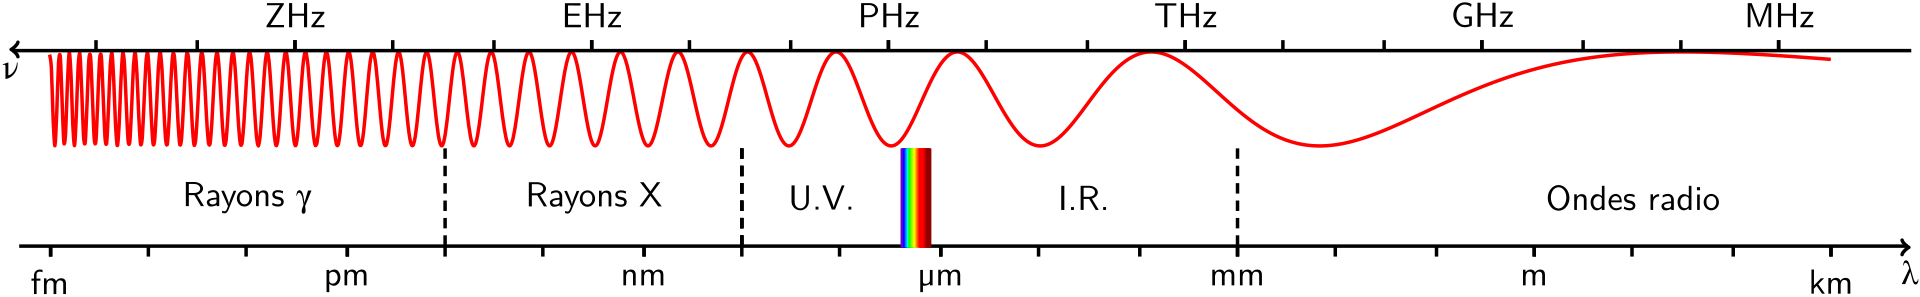
\includegraphics[width=1\linewidth]{Fig/Domaines_du_spectre_électromagnétique.png}
    \caption{Domaines du spectre électromagnétique \textit{(Par Benjamin ABEL, \href{https://commons.wikimedia.org/w/index.php?curid=22016632}{ici})}}
    \label{fig:domaine spectre electromagnetique}
\end{figure}


\subsubsection{Aspect Corpusculaire}

Si la théorie ondulatoire explique bien des phénomènes comme la diffraction ou les interférences, elle est incapable, en revanche, d'expliquer l'effet photoélectrique ou la distribution en longueur d'onde de la lumière émise par un corps chauffé (autrement dit sa couleur). \vspace{5mm}

Planck (1858-1947) a introduit la notion de discontinuité de la lumière en parlant de "photon" ("grain d'énergie") associé à la lumière.
A une radiation donnée, de fréquence $\nu$, est associé un photon (ou quantum) d'énergie:
$$\boxed{\bm{E=h\nu=\frac{hc}{\lambda}}}$$ 
\newline
$h$ est la constante de Planck; elle vaut $h=\qty{6.626e-34}{J.s}$.\newline
L'intensité de la lumière (on parle aussi de puissance radiative ou de flux photonique) est alors directement proportionnelle au nombre de photons.
L'énergie lumineuse ne peut s'échanger que par nombre entier de photons. L'énergie d'un photon est exprimée en électron-volt, c'est-à-dire l'énergie d'un électron accéléré sous une différence de potentiel de \qty{1}{Volt}; on en déduit : $\qty{1}{eV} = \qty{1,602e-19}{J}$.

Il est important de noter que lorsque la longueur d'onde augmente, l'énergie du photon associé diminue. Ces deux grandeurs sont inversement proportionnelles.\vspace{3mm}


\textbf{Exercice d'application:} Calculez $E_{(eV)}\times \lambda_{(\text{\r{A}})}$
\vspace{5mm}

\hspace{-1cm}\rotatebox[origin=b]{180}{\textbf{Réponse:\quad} $E_{(eV)}\times \lambda_{(\text{\r{A}})}=\frac{h\nu}{\qty{1.602e-19}{}\times\lambda_m}\times\lambda_{(\text{\r{A}})}=\frac{hc\lambda_{(\text{\r{A}})}}{\qty{1.602e-19}{}\times\lambda_{(\text{\r{A}})}\times10^{-10}}=\frac{\qty{6.626e-34}{}\times\qty{2.998e8}{}}{\qty{1.602e-19}{}\times10^{-10}}=12400$}
\newpage

\subsection{Spectroscopie}

La spectroscopie nécessite de disposer d'un système dispersif (prisme, réseau, ...) et d'un système détecteur (plaque photographique, photomultiplicateur, ...). Un rayonnement électromagnétique, émis par un corps excité (chauffé, éclairé, ...) peut soit: 
\begin{itemize}[label=$\ast$]
    \item comporter toutes les fréquences (spectre continu : c'est le cas de la lumière solaire) 
    \item ne comporter que quelques longueurs d'onde (spectre discontinu ou spectre de raies, c'est le cas de la lumière émise par les atomes contenus dans une vapeur métallique excitée).
\end{itemize}

\subsubsection{Spectroscopie en émission}
On cherche les caractéristiques des raies émises par une source (présentant un spectre discontinu). La position des raies sur une plaque photographique, après dispersion par un réseau ou un prisme de la lumière émise, permet par exemple de calculer leur longueur d'onde (ou leur nombre d'onde, ou leur fréquence ou leur énergie, toutes ces grandeurs étant reliées).
\begin{figure}[ht]
    \centering
    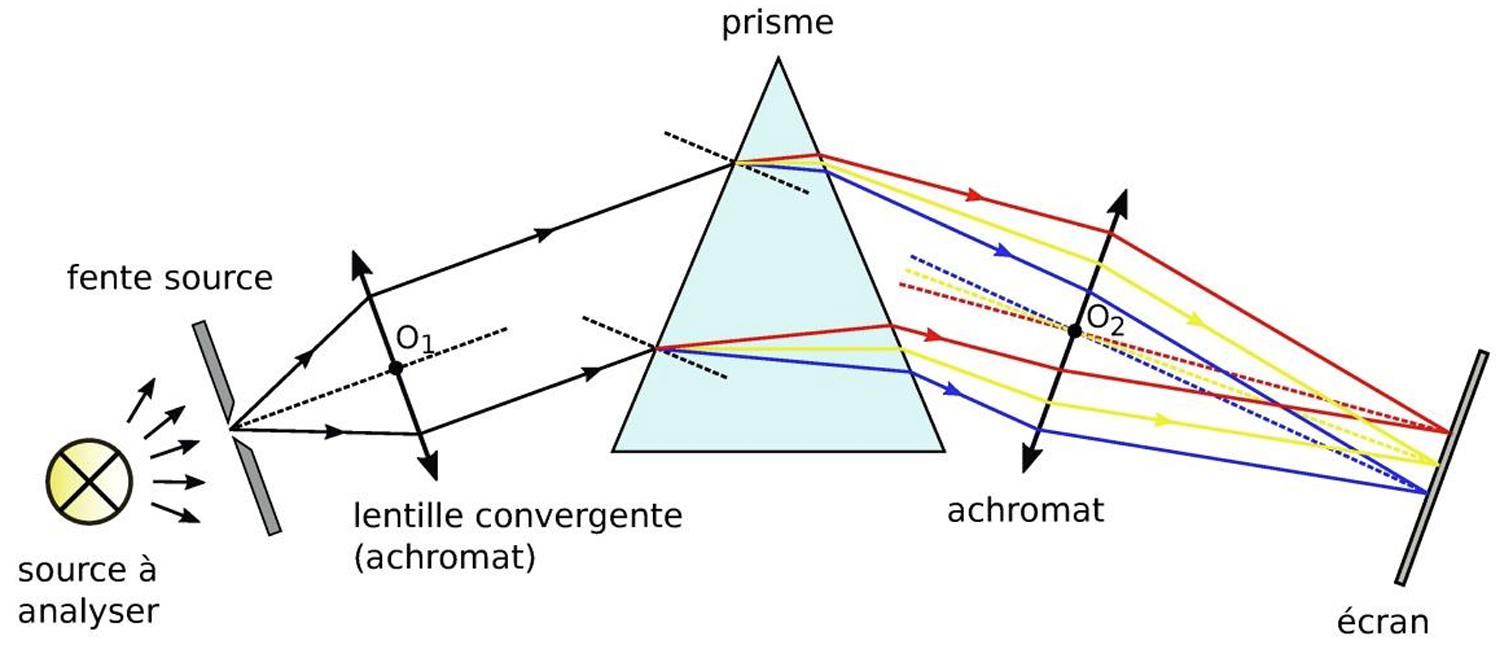
\includegraphics[width=0.75\linewidth]{Fig/Spectro-emission.png}
    \caption{Principe d'obtention d'un spectre d'émission}
    \label{fig:emission}
\end{figure}

\subsubsection{Spectroscopie en absorption}
Lorsqu'une lumière présentant un spectre continu, traverse un milieu constitué par des atomes à l'état fondamental (cas d'une vapeur métallique), elle subit des absorptions pour des longueurs d'onde bien particulières, caractéristiques du milieu traversé: il s'agit des raies d'absorption. Ces absorptions par la matière (ici les atomes du métal) entraînent un passage à l'état excité.

\begin{figure}[ht]
    \centering
    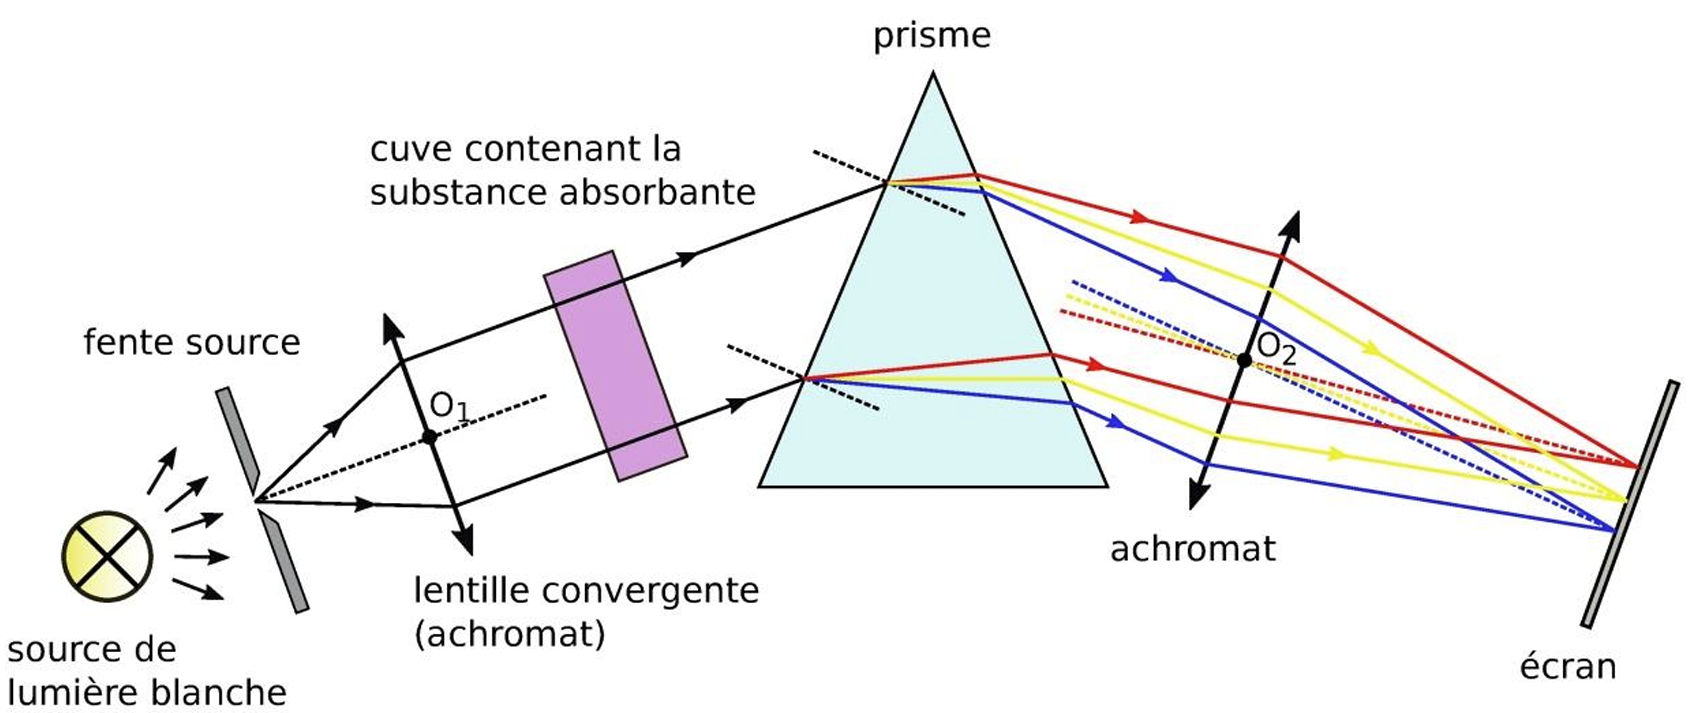
\includegraphics[width=0.75\linewidth]{Fig/Spectro-absorption.png}
    \caption{Principe d'obtention d'un spectre d'absorption}
    \label{fig:absoption}
\end{figure}

\newpage

\subsection{Résultats expérimentaux dans le cas de l'atome d'hydrogène}

C'est le cas le plus simple (Z = 1; un seul électron gravite autour du noyau). 

\subsubsection{Spectre d'absorption} 
Dans l'expérience précédente (\ref{fig:absoption}), l'échantillon est constitué de vapeur d'hydrogène monoatomique. On observe alors sur l'écran le spectre continu de la source, dont certaines fréquences (ou longueurs d'onde) sont absentes (raies sombres). L'ensemble de ces raies sombres constitue le spectre d'absorption de l'hydrogène, qui se caractérise par une série de raies situées dans l'ultraviolet lointain :  
$$\qty{900}{\angstrom} < \lambda < \qty{1250}{\angstrom}$$ 
La mesure expérimentale de la longueur d'onde de ces raies a montré qu'ils obéissent à la loi empirique: 
$$\frac{1}{\lambda} = R_H \left(1-\frac{1}{n^2}\right)$$
avec un entier $n \ge 2$, et $R_H$ une constante appelée constante de Rydberg qui vaut, pour l'hydrogène : $R_H = \qty{109677.80}{cm^{-1}}$. 

\subsubsection{Spectre d'émission}
Pour étudier le spectre d'émission de l'hydrogène, on utilise le montage expérimental de la Figure \ref{fig:emission}, en remplaçant la source par une vapeur d'hydrogène monoatomique excitée. On observe alors sur l'écran plusieurs séries de raies, dont les longueurs d'onde obéissent à nouveau à des lois empiriques. On distingue plusieurs séries: 
\begin{itemize}[label=$\ast$]
    \item la \textbf{série de Lyman} (dans l'ultraviolet): $$\frac{1}{\lambda} = R_H \left(1-\frac{1}{n^2}\right), \quad n \ge 2$$
    \item la \textbf{série de Balmer} (dans le visible): $$\frac{1}{\lambda} = R_H \left(\frac{1}{2^2}-\frac{1}{n^2}\right), \quad n \ge 3$$
    \item la \textbf{série de Paschen} (dans l'infra-rouge): $$\frac{1}{\lambda} = R_H \left(\frac{1}{3^2}-\frac{1}{n^2}\right), \quad n \ge 4$$
    \item et ainsi de suite (séries de Brackett, Pfund, etc...)
\end{itemize} \vspace{5mm}
Le spectre complet peut donc se représenter par une formule générale, empirique, dite \textbf{formule de Ritz-Balmer ou de Rydberg}:
\begin{equation}\label{Ritz-Balmer}
    \boxed{\frac{1}{\lambda} = R_H \left(\frac{1}{n'^2}-\frac{1}{n^2}\right)} 
\end{equation}
\rightline{$n,n'\in \mathbb{N} \text{\quad tels que\quad} n'<n$.}

\vspace{5mm} \noindent
Lorsque n augmente, les raies se rapprochent les unes des autres et tendent vers une raie limite $\lambda_{lim}$: 
$$\frac{1}{\lambda_{lim}}=\frac{R_H}{n'^2}$$
\newpage
Une série de raies correspond à un ensemble de raies observées dans un spectre d'émission pour lesquelles le niveau d'arrivée $n'$ est le même. La raie de tête d'une série correspond à une transition du niveau $n=n'+1$ vers le niveau $n'$. La raie limite d'une série correspond à une transition du niveau $n=+\infty$ vers le niveau $n'$. On peut représenter toutes ces transitions et niveaux d'énergie sur un diagramme de Grotrian comme celui de la Figure \ref{fig:Grotrian Hydrogene}.

\begin{figure}[ht]
    \centering
    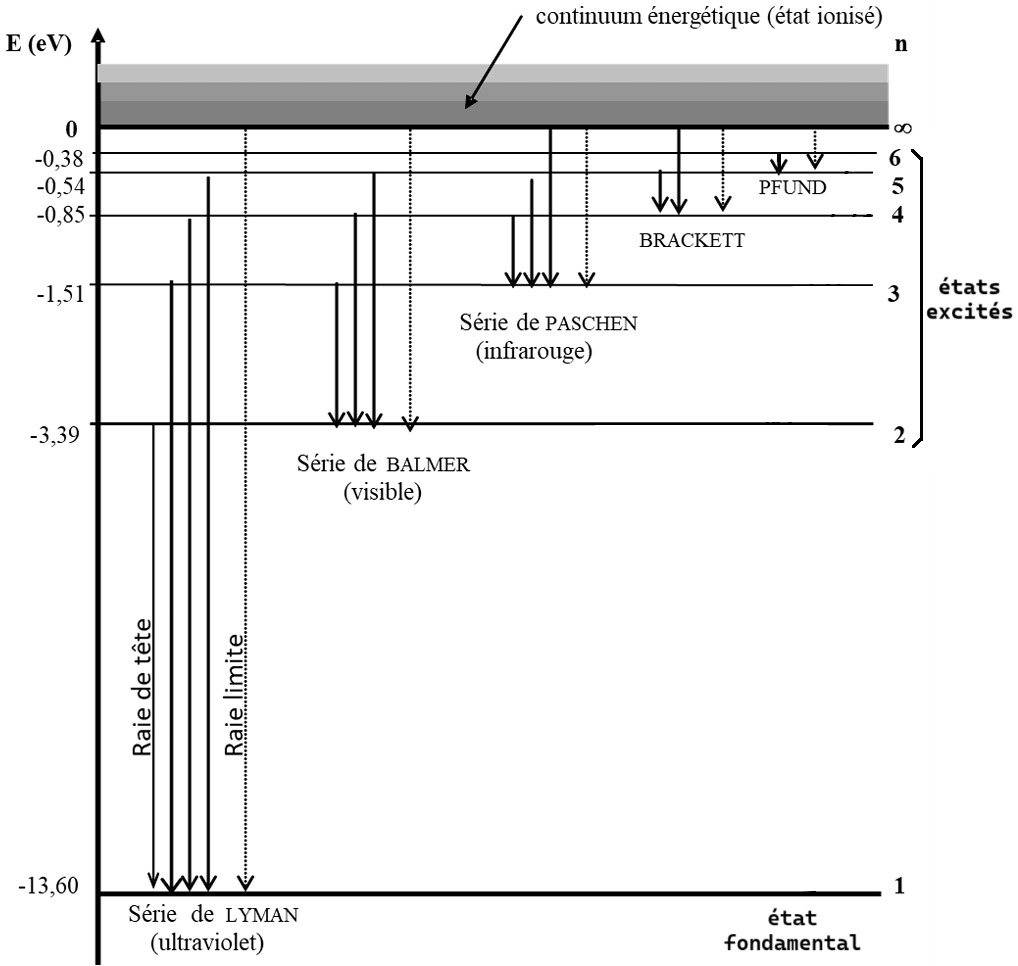
\includegraphics[width=0.75\linewidth]{Fig/Grotrian-hydrogene-v2.png}
    \caption{Diagramme de Grotrian des niveaux d'énergie de l'atome d'hydrogène }
    \label{fig:Grotrian Hydrogene}
\end{figure}

\subsection{Cas particulier des hydrogénoïdes}
Il existe un cas particulier : celui des hydrogénoïdes, c'est-à-dire des systèmes (en général des ions) qui ne possèdent qu'un seul électron : $He^+$, $Li^{2+}$, $Be^{3+}$, $B^{4+}$, ... . Dans ce cas, les nombres d'onde correspondant aux transitions observées obéissent à la loi empirique suivante, appelé \textbf{Ritz-Balmer généralisée}:
\begin{equation}\label{Ritz-Balmer generalisee}
    \boxed{\frac{1}{\lambda} = Z^2R_X \left(\frac{1}{n'^2}-\frac{1}{n^2}\right)}
\end{equation}
\hfill $n,n'\in \mathbb{N} \text{\quad tels que\quad} n'<n$.

\vspace{5mm}
les symboles $n$, $n'$ et $R_X$ ayant la même signification que précédemment, $Z$ étant le numéro atomique de l'élément considéré; $R_X$ se rapporte au système $X$ étudié. Pour les ions cités 
précédemment, $R_X$ est très voisin de $R_H$.

\newpage

\subsection*{Exercice d'application: Spectre d'émission de l'hydrogène}

\begin{figure}[h]
    \centering
    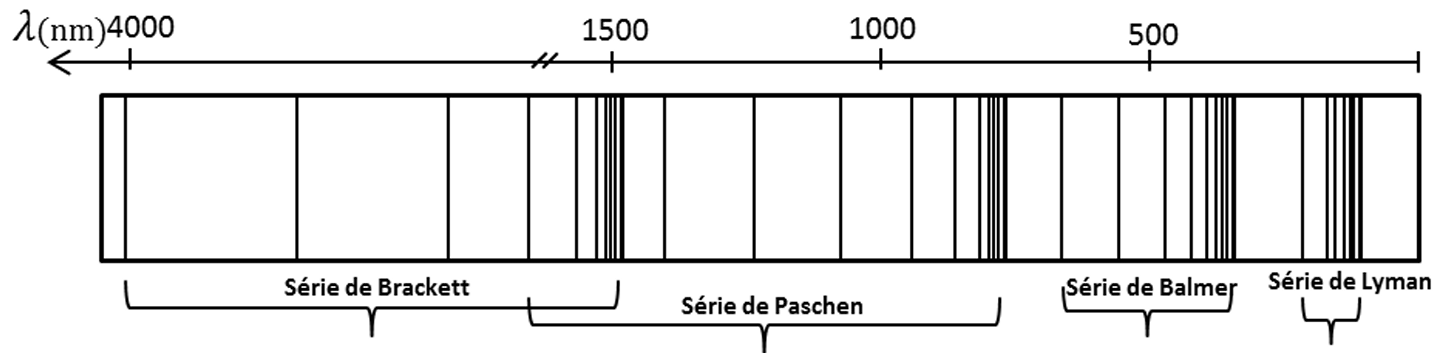
\includegraphics[width=0.9\linewidth]{Fig/Spectre-hydrogene.png}
    \caption{Spectre de l'Hydrogène}
    \label{fig:Spectre Hydrogene}
\end{figure}


\begin{enumerate}
    \item Calculez les fréquences (en $Hz$) et les longueurs d'onde (en $ \qty{}{\angstrom}$) des 4 premières raies 
    du spectre d'émission de l'hydrogène dans le visible.
    \item Quelles sont les longueurs d'onde $\lambda_{lim}$ et $\lambda_{\text{tête}}$ de la raie limite et de la raie de tête pour chacune des 
    quatre séries ($n'$ variant de 1 à 4)?
\end{enumerate}

\vspace{2.5cm}

\hspace{3.3cm}\rotatebox[origin=b]{180}{$\lambda_{\text{tête}(\qty{}{\angstrom})}= \quad n':\,$ 1: \qty{1215.7}{\angstrom} \quad 2: \qty{6564.7}{\angstrom} \quad 3: \qty{18756}{\angstrom} \quad 4: \qty{40523}{\angstrom}}

\vspace{-5mm}
\hspace{-0.4cm}\rotatebox[origin=b]{180}{$\dfrac{1}{\lambda_{\text{tête}}}= R_H \left(\dfrac{1}{n'^2}-\dfrac{1}{(n'+1)^2}\right) \quad$ D'où \quad $\lambda_{\text{tête}(\qty{}{\angstrom})}=\dfrac{10^8}{R_H \left(\dfrac{1}{n'^2}-\dfrac{1}{(n'+1)^2}\right)}=\dfrac{n'^2(n'+1)^2 \times 10^8}{R_H(2n'+1)}$}

\vspace{7mm}
\hspace{1.8cm}\rotatebox[origin=b]{180}{$\lambda_{lim(\qty{}{\angstrom})}= \quad n':\,$ 1: \qty{911.7615}{\angstrom} \quad 2: \qty{3647.046}{\angstrom} \quad 3: \qty{8205.854}{\angstrom} \quad 4: \qty{14588.18}{\angstrom}}

\hspace{3.6cm}\rotatebox[origin=b]{180}{\textbf{2.} \quad $\dfrac{1}{\lambda_{lim}}= R_H \left(\dfrac{1}{n'^2}-\dfrac{1}{"\infty"^2}\right) = \dfrac{R_H}{n'^2}$ \quad D'où \quad $\lambda_{lim(\qty{}{\angstrom})}=\dfrac{n'^2}{R_H}\times 10^8$}

\vspace{15mm}
\hspace{-0.1cm}\rotatebox[origin=b]{180}{On obtient: $n=3:$ \qty{6564.683}{\angstrom} \quad $n=4:$ \qty{4862.728}{\angstrom} \quad $n=5:$ \qty{4341.722}{\angstrom} \quad $n=6:$ \qty{4102.927}{\angstrom}}

\vspace{-0.7cm}
\hspace{0.4cm}\rotatebox[origin=b]{180}{\underline{Appli Numérique:} \quad $ \lambda_{(\qty{}{\angstrom})} = \dfrac{1\times 10^8}{\qty{109677.80}{cm^{-1}} \times \left(\dfrac{1}{4}-\dfrac{1}{n^2}\right)}$ \quad on remplace $n$ par 3, 4, 5 et 6.}

\vspace{-0.5cm}
\hspace{-0.8cm}\rotatebox[origin=b]{180}{D'où:\quad $ \lambda_{(\qty{}{\angstrom})} = \dfrac{1\times 10^8}{R_H \left(\dfrac{1}{4}-\dfrac{1}{n^2}\right)}$ \quad on multipli par $10^8$ pour obtenir le résultat en \qty{}{\angstrom} et pas en \qty{}{cm^{-1}}. }

\hspace{4.8cm}\rotatebox[origin=b]{180}{On a donc d'après Ritz-Balmer: $ \dfrac{1}{\lambda} = R_H \left(\dfrac{1}{2^2}-\dfrac{1}{n^2}\right), \quad n \ge 3 $.}

\vspace{2mm}
\hspace{-2.4cm}\rotatebox[origin=b]{180}{\textbf{1.} \quad Les raies d'émissions du spectre de l'hydrogène dans le visible correspondent à la série de Balmer (cours).}

\vspace{5mm}
\hspace{13cm}\rotatebox[origin=b]{180}{\textbf{Réponse:}}


\newpage


\subsection{Le modèle de Bohr pour l'atome d'hydrogène}
\noindent Le modèle le plus simple permettant d'expliquer les résultats expérimentaux présentés ci-dessus,
est le modèle de Bohr (1913) pour l'atome d'hydrogène.
Il repose sur trois hypothèses majeures: 
\begin{itemize}[label=$\ast$]
    \item l'électron (masse $m$) de l'atome d'hydrogène gravite autour du noyau
    sur une trajectoire circulaire de rayon $r$, à la vitesse $v$.

    L'énergie totale de l'électron est proportionnelle à la distance $r$ entre l'électron et le noyau.
    \textbf{Cette énergie est négative !}

    \item Seules certaines valeurs de $r$ sont admises en raison de la quantification du moment cinétique de l'électron.
    $$r=\frac{\varepsilon_0 h^2}{\pi me^2}n^2\, ,\quad \text{avec $n$ entier.}$$
    Ainsi, \textbf{l'énergie de l'électron est quantifiée} puisqu'elle dépend du rayon $r$.
    
    \textbf{Le nombre entier $\bm{n}$ est appelé nombre quantique principal.}
        \vspace{5mm}
    \item  Lorsque l'électron se déplace sur une orbite de rayon bien défini ($r$ constant),
    il ne rayonne pas d'énergie ; on dit qu'il se trouve dans un état stationnaire.
    \textbf{Toute variation de l'énergie de l'électron respecte la théorie des quanta:}
    toute absorption ou émission d'un rayonnement ne peut avoir lieu que sous forme de
    multiples entiers d'une quantité minimale d'énergie égale à un quantum.
    
    En l'absence d'excitation, l'électron de l'hydrogène est dans son état de plus basse énergie,
    appelé état fondamental, caractérisé par $n=1$.
    Une excitation conduit l'électron à occuper un état d'énergie plus élevé,
    \textbf{appelé état excité}. Il occupe alors une trajectoire plus éloignée du noyau.
    Pour une transition entre un niveau d'énergie $E_n$ et un niveau d'énergie $E_n'$: 
    $$\frac{1}{\lambda}=\frac{me^4}{8\varepsilon_0^2h^3c}\left| \frac{1}{n^2}-\frac{1}{n'^2}\right|$$ 
    On retrouve la formule de Ritz-Balmer (\ref{Ritz-Balmer generalisee}) avec $R_\infty=\dfrac{me^4}{8\varepsilon_0^2h^3c} \approx R_H$ .
\end{itemize}

\subsection{Limites de la théorie de Bohr}
\noindent Le modèle de Bohr n'est pas capable d'expliquer 3 phénomènes expérimentals:
\begin{itemize}[label=$\ast$]
    \item les raies ne sont pas simples mais correspondent à un ensemble de raies de longueurs
    d'onde très voisines.
    \item placé dans un champ magnétique ou un champ électrique intense,
    un atome d'hydrogène voie son spectre d'émission modifié.
    \item les atomes polyélectroniques ne peuvent pas être décrit par le modèle de Bohr.
\end{itemize}

\noindent Donc, même si le modèle de Bohr présente un intérêt certain pour une représentation 
simple de l'atome d'hydrogène, il est nécessaire d'envisager une autre description de l'atome: c'est ce que propose \textbf{le modèle ondulatoire}. 


\section{Le Modèle Ondulatoire de l'atome}

\subsection{Édification de la mécanique quantique}

Les modèles "classiques" de l'atome étant incapables d'expliquer correctement le
comportement microscopique de la matière, il était nécessaire de définir les bases
d'une \textbf{nouvelle théorie se devant de concilier le
double aspect ondulatoire et corpusculaire de la matière et du rayonnement.} 

De plus, cette théorie se devait de retrouver la mécanique classique comme limite
et être applicable essentiellement aux systèmes microscopiques
(molécules, atomes, électrons \dots). 

\textbf{Si un quantum $h\nu$ ($h = \qty{6,626e-34}{J.s}$) a un effet non mesurable
sur un système (systèmes macroscopiques), alors une description
"classique" des phénomènes est suffisante.} Par contre, \textbf{si ce même quantum provoque un
effet important sur un système (cas des atomes et des molécules) alors la description quantique est indispensable.}

\subsection{Relation de Bröglie}

Les électrons sont en général considérés comme des particules, puisqu'ils possèdent
une masse. Cependant, il est également possible d'obtenir la diffraction d'un faisceau
d'électrons comme on peut le faire avec une radiation électromagnétique. 

Ainsi, Louis de Bröglie (en 1924) a proposé d'\textbf{étendre à toute particule microscopique de masse $\bm{m}$ se déplaçant à une
vitesse $\bm{v}$ cette dualité onde-corpuscule bien établie pour le photon}.
Ainsi, à la particule, on peut associer une longueur d'onde $\lambda$ telle que:
$$\lambda=\frac{h}{mv}=\frac{h}{p}$$
Pour les photons qui ont une masse nulle, on utilise leur quantité de mouvement $p$.


\subsection{Notion d'orbitale}

\subsubsection{Principe d'indétermination d'Heisenberg}

Dans le modèle de Bohr de l'hydrogène, la position de l'électron et sa vitesse sont
parfaitement déterminées.\textbf{Dans la théorie quantique, la position et la vitesse
ne sont pas déterminés.}
On peut déterminer une région de l'espace et un intervalle de vitesse
dans lesquels l'électron a une certaine probabilité de se trouver.
La relation d'Heisenberg stipule que les incertitudes
$\Delta x$ et $\Delta (mv)$ sont liées par la relation:
$$\Delta x \Delta(mv) \ge \frac{h}{4\pi}$$

Ainsi, si la position est connue avec précision ($\Delta x$ faible) alors
la vitesse est affectée d'une grande incertitude ($\Delta (mv)$ grand), et réciproquement.
\textbf{L'objet quantique n'a plus de localisation ni de vitesse parfaitement déterminée}.


\subsubsection{Densité de probabilité de présence dans l'orbitale}

Le manque d'information sur la vitesse ou la position de l'électron nécessite
l'introduction de la notion de probabilité de trouver l'électron à une position donnée.
On appelle cela la densité électronique, ou densité de probabilité de présence en ce point.
\textbf{Une orbitale atomique est un espace délimité qui donne la probabilité de présence
d'un électron.}

On la représente ainsi souvent à l'aide de surfaces qui délimitent la région à
l'intérieur de laquelle la probabilité de présence de l'électron est supérieure
à un seuil donné (par exemple 90 \%).

\subsubsection{Fonction d'onde et quantification d'énergie}

L'équation de Schrödinger lie l'énergie d'un électron et sa probabilité de présence
en différents points, avec la fonction d'onde $\Psi(x, y, z)$:
$$H\footnote{$H$ est un opérateur mathématique (Hamiltonien).}\Psi = E\Psi$$

Les solutions à cette équation sont chacune une fonction d'onde $\Psi$, caractérisée
par une valeur particulière, quantifiée, de $E$. 
$\Psi^2$ représente la densité électronique au point $M(x,y,z)$. 

La notion d'orbitale introduite précédemment englobe ainsi la fonction d'onde et l'énergie qui lui correspond.

\noindent
Cette fonction d'onde $\Psi$ à des \textbf{conditions aux limites :}
\begin{itemize}[label=$\ast$]
    \item La probabilité de présence de la particule en un point de l'espace ne peut prendre qu'une seule valeur. 
    \item la probabilité de présence de la particule ne peut pas présenter de discontinuité. 
    \item en explorant tout l'espace, la probabilité de présence doit être égal à 1 (condition de normation). 
\end{itemize}

\subsubsection{Les nombres quantiques}

Chaque solution de l'équation de Schrödinger correspond à une valeur quantifiée de
l'énergie et ne peut être obtenue que par la prise en compte de trois nombres quantiques
qui lui sont spécifiques: $n$, $l$  et $m_l$  (Tableau \ref{tab:Caractéristiques des trois nombres quantiques}).

\begin{table}[h]
    \centering
    \begin{tabular}{|c|c|c|}
    \hline
        \textbf{Symbole} & \textbf{Nom}  & \makecell{\textbf{Valeurs possibles} \\ $\pmb{n,l,m_l \in \mathbb{N}}$} \\ \hline
        $\bm{n}$ & principal & $n\ge 1$ \\ \hline
        $\bm{l}$ & secondaire (ou azimutal) & $0 \le l \le n-1$ \\ \hline
        $\bm{m_l}$ & magnétique orbital & $-l \le m_l \le +l$ \\ \hline
    \end{tabular}
    \caption{Caractéristiques des trois nombres quantiques}
    \label{tab:Caractéristiques des trois nombres quantiques}
\end{table}

\begin{itemize}[label=$\ast$]
    \item $\bm{n}:$ Nombre quantique principal. Lié à la "taille" de l'orbitale. Numérote la couche électronique.

    \item $\bm{l}:$ Nombre quantique secondaire. Lié à la forme de
    l'orbitale. Numérote la sous-couche. 

    \item $\bm{m_l}:$ Nombre quantique orbital (ou magnétique).
    Lié à l'orientation de l'orbitale.
    Le nombre de valeurs possible de $m_l$ correspond au nombre d'orbitales sur une sous-couche $l$.
\end{itemize}

\subsubsection{Nomenclature et représentation des orbitales}

\begin{wraptable}[5]{r}{0.4\textwidth}
    \centering
    \vspace{-1cm}
    \begin{tabular}{|c|c|c|c|c|}
    \hline
    \diagbox{$\bm{l}$}{$\bm{n}$} & $\bm{1}$ & $\bm{2}$ & $\bm{3}$ & $\bm{4}$ \\ \hline
    $\bm{0}$ & $1s$ & $2s$ & $3s$ & $4s$ \\ \hline
    $\bm{1}$ & - & $2p$ & $3p$ & $4p$ \\ \hline
    $\bm{2}$ & - & - & $3d$ & $4d$ \\ \hline
    $\bm{3}$ & - & - & - & $4f$ \\ \hline
    \end{tabular}
    \caption{Noms des orbitales en fonction de $n$ et $l$}
    \label{tab:nom des sous-couches}
\end{wraptable}

Les orbitales sont nommées (comme les sous-couches électroniques) d'après les valeurs
des nombres quantiques. La première partie du nom est le nombre quantique principal,
la seconde partie est liée au nombre quantique secondaire
(Tableau \ref{tab:nom des sous-couches}).

\vspace{2cm}
\begin{table}[h]
    \centering
    \begin{tabular}{|c|c|c|c|}
    \hline
    \makecell{\textbf{Nombre quantique} \\ \textbf{secondaire} \bm{$l$}} & \makecell{\textbf{Nom de la} \\ \textbf{sous-couche}} & \makecell{\textbf{Nombre} \\ \textbf{d'orbitales}} & \textbf{Origine du nom} \\ \hline
    0 & $s$ & 1 & sharp \\ \hline
    1 & $p$ & 3 & principal \\ \hline
    2 & $d$ & 5 & diffuse \\ \hline
    3 & $f$ & 7 & fundamental \\ \hline
    \end{tabular}
    \caption{Nombre d'orbitales par sous-couches}
    \label{tab:nombres d'orbitales}
\end{table}


\vfill
\noindent\textbf{Exercice d'application:} Déterminez le nombre de cases quantiques et d'électrons que peut contenir une sous-couche $p$, $d$ puis $f$.

\rotatebox[origin=b]{180}{$f$: $l=3$ donc $m_l\{-3,-2,-1,0,1,2,3\}$. IL y a 7 cases quantiques. 14 électrons max.}

\rotatebox[origin=b]{180}{$d$: $l=2$ donc $m_l\{-2,-1,0,1,2\}$. IL y a 5 cases quantiques donc 10 électrons max.\hspace{1mm}}

\rotatebox[origin=b]{180}{\textbf{Réponse:} $p$: $l=1$ donc $m_l=\{-1,0,1\}$. Il y a 3 cases quantiques donc 6 électrons maximum.}

\clearpage

\noindent Il existe plusieurs façons de représenter une orbitale:
\begin{itemize}[label=$\ast$]
    \item Tracer des surfaces d'isodensité électronique, constituées de l'ensemble des points de l'espace en lesquels la densité de probabilité de présence a la même valeur (Voir \ref{fig:densité de proba}).

    \item Tracer des surfaces d'isodensité électronique délimitant des volumes à l'intérieur desquels la probabilité de présence de l'électron a une certaine valeur ($50\%$, $95\%$ par exemple) (Voir \ref{fig:contour proba}).
    
\end{itemize}

\begin{figure}[ht]
    \centering
    \begin{subfigure}{0.45\textwidth}
        \centering
        \includegraphics[width=0.8\linewidth]{Fig/densité-proba.jpg}
        \caption{Densité de probabilité de l'électron}
        \label{fig:densité de proba}
    \end{subfigure}
    \hfill\begin{subfigure}{0.45\textwidth}
        \centering
        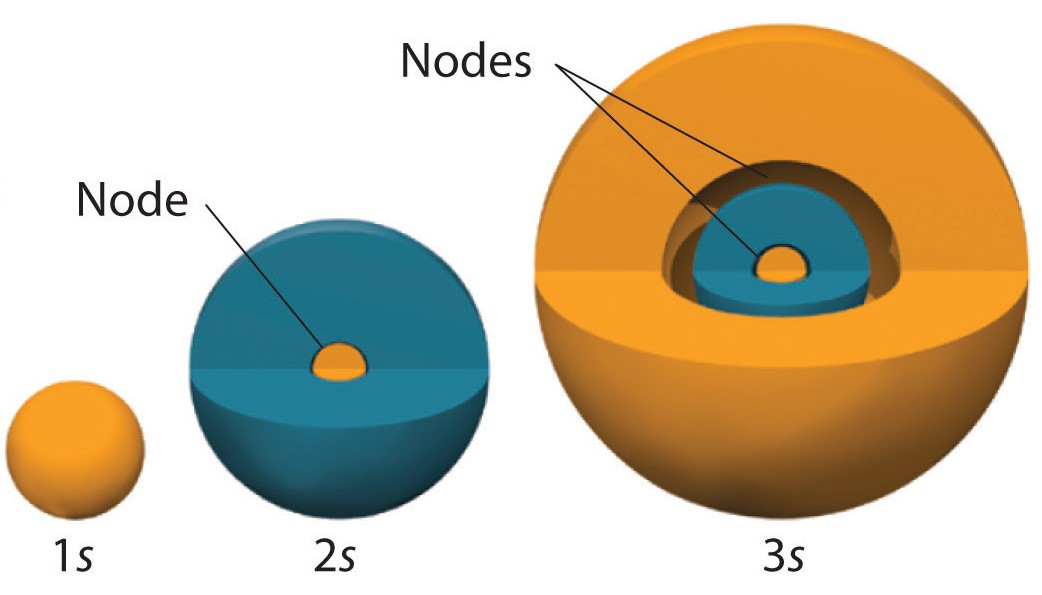
\includegraphics[width=0.8\linewidth]{Fig/contour-proba.jpg}
        \caption{Probabilité de présence de l'électron dans un volume}
        \label{fig:contour proba}
    \end{subfigure}
\end{figure}

\begin{figure}[h]
    \centering
    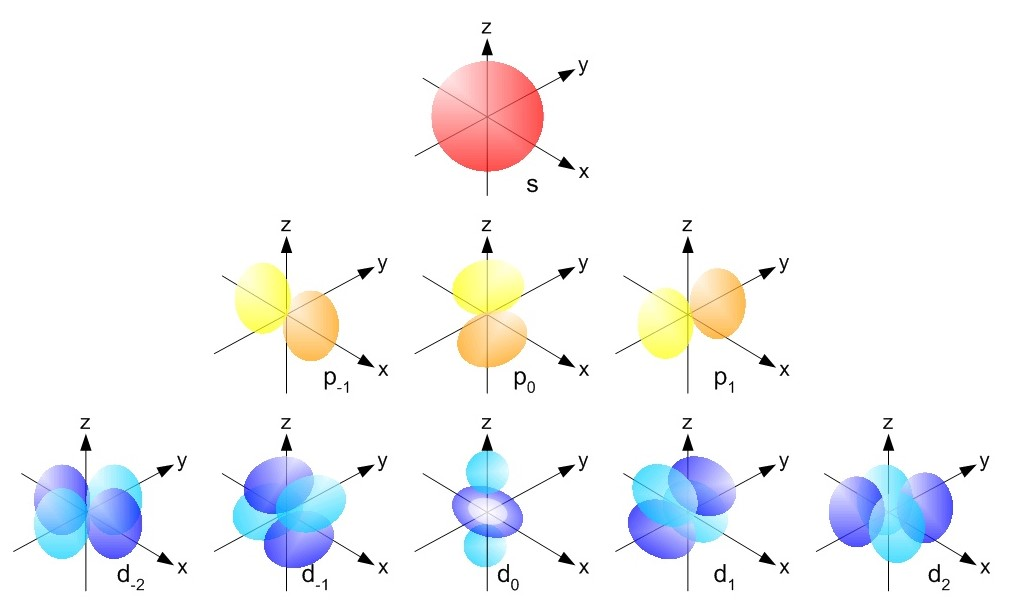
\includegraphics[width=0.8\linewidth]{Fig/orbitales.jpg}
    \caption{Représentation des orbitales $s$ à $d$}
    \label{fig:Représentation des orbitales}
\end{figure}

\begin{itemize}[label=$\ast$]
    \item Tracer des cases quantiques qui représentent chacune une orbitale constituée
    au maximum de deux électrons. Chaque triplet de valeur $(n, l, m_l)$ a une case
    quantique associée. Les flèches représentent les électrons et leur spin (Voir \ref{section: spin}).
\end{itemize}

\begin{center}
\electron{3s}{\updwn}\quad \electron{3p}{\updwn\ \updwn\ \updwn} \quad \electron{3d}{\updwn\ \updwn\ \updwn\ \haut\ \haut}
\end{center}


\subsubsection{Le nombre de spin}\label{section: spin}

\begin{wrapfigure}[9]{r}{0.3\textwidth}
    \centering
    \vspace{-1.5cm}
    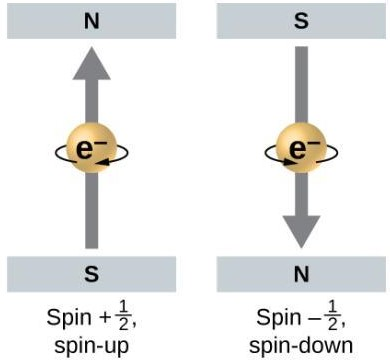
\includegraphics[width=0.3\textwidth]{Fig/spin.jpg} 
    \caption{Spin d'un électron}
    \label{fig:spin}
\end{wrapfigure}
Chaque orbitale ne peut être occupée que par deux électrons au maximum. Lorsque deux électrons occupent une orbitale, on différencie ces électrons par leur nombre de spin $s$ (ou $m_s$), \textbf{qui traduit la quantification de leur moment cinétique intrinsèque (représentatif du mouvement de rotation de l'électron sur lui-même) ou encore l'orientation de l'électron dans un champ magnétique.}

Il ne peut prendre que deux valeurs: $s=\pm \frac{1}{2}$



\section{Atomes Polyélectroniques - Configuration électronique}

\subsection{Approximation monoélectronique, charge nucléaire effective}

Contrairement aux atomes monoélectroniques, un électron d'un atome polyélectronique interagit à la fois avec le noyau et les autres électrons qui l'entourent (interaction électrostatique).

Les niveaux d'énergie sont démultipliés, car décomposés par la présence d'électrons entre le noyau et l'électron considéré, qui est perçue différemment selon le type d'orbitale à laquelle appartient l'électron. Par exemple, comme le montre la Figure \ref{fig:Densité de probo radiale orbitale 3s 3p 3d} ci-dessous, un électron $3s$ ressentira davantage la charge du noyau qu'un électron $3p$ ou $3d$; on dit alors que l'orbitale $3s$ est plus pénétrante que l'orbitale $3p$ (ou $3d$).

\begin{figure}[ht]
    \centering
    \includegraphics[width=0.5\linewidth]{Fig/Densité de probo radiale orbitale 3s 3p 3d.png}
    \caption{Densité de probabilité radiale pour les orbitales $3s$, $3p$, $3d$}
    \label{fig:Densité de probo radiale orbitale 3s 3p 3d}
\end{figure}

Au plan théorique, la résolution rigoureuse de l'équation de Schrödinger s'avère impossible. On est ainsi amené à faire des hypothèses simplificatrices. Dans l'approximation monoélectronique, pour un électron donné, on remplace l'ensemble (noyau + autres électrons) par une charge nucléaire effective $Z^*$. 

\textbf{La charge nucléaire effective est la charge d'un noyau fictif
qui exercerait sur un électron, en l'absence des autres électrons,
la même influence que l'ensemble réel (noyau de charge $Z$ + autres
électrons)}. Les autres électrons exercent donc, sur un électron particulier,
un effet d'écran représenté par une constante d'écran $\sigma$.
C'est l'hypothèse de Slater, qui permet d'estimer des valeurs de $Z^*$ sachant que
$Z^* = Z - \sigma$.

\begin{collect*}{mytable}{\setcounter{duptable}{\value{table}}}{}{}{}
\begin{table}[h]
    \centering
    \begin{tabular}{|c|c|c|c|c|}
     \hline
        \textbf{Orbitale de l'électron} & $n'<n-1$ & $n'=n-1$ & $n'=n$ & $n'>n$ \\ \hline
        $\bm{1s}$ & 1.00 & 0.85 & 0.30 & 0 \\ \hline
        $\bm{ns, np}$ & 1.00 &  0.85 & 0.35 & 0 \\ \hline
        $\bm{nd}$ & 1.00 & 1.00 & \makecell{1.00 pour $s$ et $p$ \\ 0.35 pour $d$} & 0 \\ \hline
    \end{tabular}
    \caption{Contributions des électrons des orbitales selon la règle de Slater}
    \label{tab:Contributions des électrons des orbitales selon la règle de Slater}
\end{table}
\end{collect*}

\subsection{Organisation du nuage atomique}

\subsubsection{Le nuage électronique}

L'ensemble des électrons ayant la même valeur de $n$ constitue une couche électronique; des symboles ont été attachés aux valeurs de $n$ caractérisant les couches (Tableau \ref{tab:symboles associes couches}).

\begin{table}[h]
    \centering
    \begin{tabular}{|c|c|c|c|c|c|c|}
        \hline
        $\bm{n}$ & 1 &  2 & 3 & 4 & 5 & 6 \\ \hline
        \textbf{Symbole} & K & L & M & N & O & P \\ \hline
    \end{tabular}
    \caption{Symboles attachés aux différentes couches}
    \label{tab:symboles associes couches}
\end{table}

A l'intérieur d'une couche donnée ($n = cste$), les électrons sont répartis en différents types de sous-couches, caractérisées par différentes valeurs du nombre quantique secondaire $l$. Des symboles sont attachés à ces sous-couches (Voir \ref{tab:nom des sous-couches}). On retrouve à l'intérieur des sous-couches des \textbf{orbitales} ou \textbf{cases quantiques} associées aux valeurs possible de $m_l$. Voir le tableau \ref{tab:nombres d'orbitales} qui dénombre le nombre de cases quantiques par sous-couche (Il y a maximum deux fois plus d'électrons que de cases quantiques).

\newpage

\subsubsection{La configuration électronique}

L'arrangement énergétique des électrons dans l'atome fait appel à plusieurs règles.
\textbf{Le principe général est, à l'état fondamental, d'occuper tous les états de plus basse énergie},
il n'est donc pas possible de disposer tous les électrons de façon quelconque et 3
règles ont été établis:

\begin{itemize}[label=$\ast$]
    \item \textbf{Principe de Pauli:} "Un atome ne peut pas avoir deux électrons ayant
    les 4 mêmes nombres quantiques ($n$, $l$, $m_l$ et $m_s$)".
    Il ne peut y avoir que 2 électrons par cases quantiques (ou orbitales).\\
    Case vide: \electron{}{\emp} \quad Case à demi remplie: \electron{}{\haut} \quad Case pleine: \electron{}{\updwn}

    \item \textbf{Règle de Klechkowski:} Les niveaux sont remplis par ordre d'énergie
    croissante. La technique consiste à faire un remplissage à ($n + l$) croissant et,
    pour deux mêmes valeurs de ($n + l$), à $n$ croissant. Voir \ref{fig:Règle de Klechkowski}.
    \item \textbf{Règle de Hund:} Le fait d'apparier des électrons de spin opposé
    coûte de l'énergie; il en découle que toutes les orbitales d'une sous-couche
    doivent être occupées chacune par un électron célibataire avant que l'une d'elles
    puisse être occupée par deux électrons appariés. Les électrons célibataires sont nécessairement à spins parallèles. 
    \begin{center}
            \electron{3p}{\haut \ \haut \ \haut}  \hspace{3mm} {\Large $^{\text{puis}}$} \hspace{3mm}\electron{3p}{\updwn \ \haut \ \haut}
    \end{center}
    \item \textbf{Exceptions aux règles de remplissage:} Il existe des exceptions à la
    règle de Klechkowski en raison de la stabilité de certaines sous-couches à
    demies-remplies ou totalement remplies. Par exemple, au lieu d'avoir
    $3d^4\,4s^2$ on aura $3d^5\,4s^1$ pour le Chrome (Cr) ou encore on aura $4s^1\,3d^10$ au lieu de $4s^2\,3d^9$.
\end{itemize}

\begin{figure}[h]
    \centering
    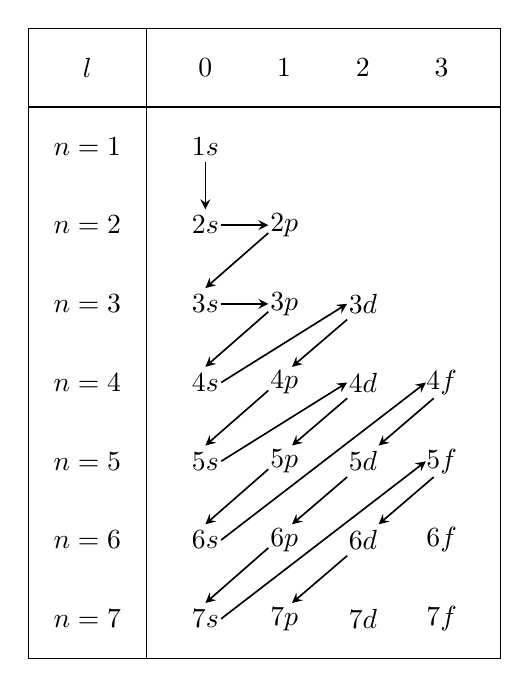
\begin{tikzpicture}
        % Style pour les flèches
        \tikzstyle{arrow} = [semithick,->,>=stealth]

        % Ajout des étiquettes pour n (niveau) à gauche
        \foreach \n in {1,..., 7}{
            \node at (-1.5,-\n+1) {$n=\n$};
        }
        % Ajout des étiquettes pour l (valeur de sous-couche) en haut
        \node at (-1.5,1) {$l$};
        \foreach \n in {0,...,3}{
        \node at (\n,1) {$\n$};
        }
    
        % Dessin des lignes de séparation horizontales pour n
        \draw[] (-2.25,1.5) -- (3.75,1.5);
        \draw[] (-2.25,0.5) -- (3.75,0.5);
        \draw[] (-2.25,-6.5) -- (3.75,-6.5);
    
        % Dessin des lignes de séparation verticales pour l
        \draw[] (-2.25,1.5) -- (-2.25,-6.5);
        \draw[] (-0.75,1.5) -- (-0.75,-6.5);
        \draw[] (3.75,1.5) -- (3.75,-6.5);
    
        % Positionnement des sous-couches sans contour
        \foreach \n in {1,...,7}{
        \node at (0,-\n+1) {$\n s$};}
         \foreach \n in {2,...,7}{
        \node at (1,-\n+1) {$\n p$};}
         \foreach \n in {3,...,7}{
        \node at (2,-\n+1) {$\n d$};}
         \foreach \n in {4,...,7}{
        \node at (3,-\n+1) {$\n f$};}

        % Dessin des flèches suivant la règle de Klechkowski
        \draw[arrow] (0,-0.2) -- (0,-0.8);       % 1s -> 2s
        \draw[arrow] (0.2,-1) -- (0.8,-1);       % 2s -> 2p
        % fleches p à s
        \foreach \n in {1,...,5}{
        \draw[arrow] (0.8,-\n-0.1) -- (0,-\n-0.8);}
        % fleche p à d
        \foreach \n in {2,...,5}{
        \draw[arrow] (1.8,-\n-0.2) -- (1.1,-\n-0.8);}
        \draw[arrow] (0.2,-2) -- (0.8,-2);       % 3s -> 3p
        \draw[arrow] (0.2,-3) -- (1.8,-2);       % 4s -> 3d
        \draw[arrow] (0.2,-4) -- (1.8,-3);       % 5s -> 4d
        \draw[arrow] (0.2,-5) -- (2.8,-3);       % 6s -> 4f
        \draw[arrow] (2.9,-3.2) -- (2.2,-3.8);   % 4f -> 5d
        \draw[arrow] (0.2,-6) -- (2.8,-4);       % 7s -> 5f
        \draw[arrow] (2.9,-4.2) -- (2.2,-4.8);   % 5f -> 6d
        
    \end{tikzpicture}

    \caption{Règle de Klechkowski}
    \label{fig:Règle de Klechkowski}
\end{figure}

\subsubsection{Les électrons de valences}

Les électrons de valence d'un atome sont: 
\begin{itemize}[label=$\ast$]
    \item Les électrons de plus grand nombre quantique principal $n$.
    \item Les électrons d'une sous-couche ($n$ inférieur) non totalement remplie.
\end{itemize} 

Ce sont ces électrons qui pourront être mis en jeu dans la formation des liaisons covalentes
(cf chapitre \ref{sec:Liaison covalente}).



\section{Classification Périodique des Elements}

\subsection{Présentation}

La classification périodique moderne classe les éléments par numéro atomique $Z$ croissant (pas par masse atomique croissante). Elle fait apparaître un peu plus de $100$ éléments dont $90$ (de $Z=1$ à $Z=92$ exception faite de $Z=43$ et $Z=61$) existent dans la nature. Les autres ont été préparés artificiellement. 

\subsection{Les périodes}

Parmi les dispositions possibles pour présenter la classification périodique, nous nous bornerons au tableau à 18 colonnes, qui est le plus courant. Dans cette présentation, les lanthanides (de la $6^{\text{ème}}$ période) et les actinides (de la $7^{\text{ème}}$ période) sont reportés au bas du tableau. 

\subsection{Les colonnes (ou familles)}

\pgfPTbuildcell(5,3)[(1;1-2;Z),(2-3;1-3;CS),(4-5;1-3;name)]
\hspace{0.5cm}\pgfPT[
    CS all=darkgray,    
    cell size=22pt, 
    show families, 
    families font color=black,
    show title=false, 
    show legend=false,
    families font=\tiny,
    name font=\Tiny
    ]


\subsubsection{Eléments du groupe principal}

\begin{itemize}[label=$\ast$]
    \item  \textbf{les alcalins} (groupe 1), structure électronique externe en ($ns^1$).
    \item  \textbf{les alcalino-terreux} (groupe 2), structure électronique externe en ($ns^2$).
    \item \textbf{les chalcogènes} (groupe 16), structure électronique externe en ($ns^2, np^4$).
    \item \textbf{les halogènes} (groupe 17), structure électronique externe en ($ns^2, np^5$). 
    Eléments très réactif (d'où leurs dangerosités).
    \item les autres groupes (13 à 15) du bore à l'azote ($ns^2, np^1$) à ($ns^2, np^3$)
\end{itemize}

\subsubsection{Les gazs rares}

Dernière colonne du tableau, (groupe 18). On les appelle aussi \textbf{gaz nobles} ou gaz "inertes".
Toutes les couches sont saturées. A l'exception du premier (He : $1s2$),
leur structure électronique externe est ($ns2, np6$) les rends très peu réactif.

\subsubsection{Les éléments de transition}

Les deux couches externes ne sont ni saturées, ni pseudo-saturées. Ils sont 
caractérisés par un niveau $d$ dans l'avant dernière couche non complètement rempli ($n-1$). 
Les électrons de la dernière couche ($ns$) y sont faiblement retenus. Les propriétés chimiques de ces éléments varient peu entre eux.


\subsubsection{Les lanthanides et les actinides: éléments de transition interne}

Les 3 couches externes ne sont ni saturées, ni pseudo-saturées. Ces éléments sont 
caractérisés par un niveau $f$ non complètement rempli dans l'antépénultième couche. 
Les propriétés chimiques seront pratiquement les mêmes pour tous les lanthanides (appelés parfois terres rares) et pour tous les actinides. 


\subsection{Les blocs}
On découpe souvent le tableau en "blocs" comme on le voit sur le tableau ci-dessous:
\vspace{5mm}

\hspace{0.5cm}\pgfPT[
    CS all=darkgray,    
    csBlocks,
    blocks font color=black,
    cell size=22pt, 
    show blocks, 
    show title=false, 
    show legend=false,
    blocks font=\small,
    name font=\Tiny
    ]

\begin{itemize}[label=$\ast$]
    \item \textbf{le bloc s} regroupe les colonnes 1 et 2.
    \item  \textbf{le bloc p} regroupe les colonnes 13 à 18.
    \item  \textbf{le bloc d} regroupe les colonnes 3 à 12.
    \item  \textbf{le bloc f} regroupe les lanthanides et les actinides.
\end{itemize}




\section{Propriétés physiques des éléments}

\subsection{Rayon atomique}

$ r \propto \dfrac{n^2}{Z^*} \quad n$ correspond à la période.

\vspace{3mm}
\hspace{0cm}\pgfPT[
    Z list=spd,
    CS all=darkgray,    
    csSoft,
    cell size=22pt, 
    show title=false, 
    show legend,
    show legend pins=false,
    name font=\Tiny,
    show periodic variations,
    cell style=pgfPTR,
    varR font=\footnotesize
    ]


\subsection{Energie d'ionisation}

C'est l'énergie qui correspond à la réaction: $A_{(gaz)} \rightarrow A^+_{(gaz)} + e^-$

Le deuxième ionisation demande plus d'énergie (ainsi de suite pour la $n^{\text{ème}}$): 
$$A^{+}_{(gaz)} \rightarrow A^{2+}_{(gaz)} + e^-$$

\vspace{1mm}
\hspace{0cm}\pgfPT[
    Z list=spd,
    CS all=darkgray,    
    csSoft,
    cell size=22pt, 
    show title=false, 
    show legend,
    show legend pins=false,
    name font=\Tiny,
    show periodic variations,
    cell style=pgfPTEi,
    varEi font=\footnotesize,    
    varR font=\footnotesize,
    varEi color=purple!50!white,
    Ei color=purple
    ]


\subsection{Electronégativité} \label{sous-section:Electronégativité}

\textbf{L'électronégativité correspond à la tendance qu'a un élément à attirer vers lui un doublet de liaison.} L'électropositivité sera la tendance inverse.
On note que l'électronégativité du fluor, élément le plus électronégatif, est égale à 4, celle 
du césium, élément le moins électronégatif, à 0,7 et celle de l'hydrogène à 2,1.
Voir le tableau \ref{fig:Electronégativité} sur la $3^{\text{ème}}$ de couverture.



\section{Spectroscopie des Rayon X}

\subsection{Nature et production des Rayons X}

Les rayons X sont des radiations électromagnétiques comme la lumière, mais d'une 
longueur d'onde bien plus courte ($<10 nm$), ce qui correspond à des 
énergies supérieures (\qty{0.1}{keV} à \qty{}{MeV}).

La source de rayons X la plus utilisée est le tube à rayons X (Figure \ref{fig:tube à rayons X}) qui comprend:

\begin{itemize}[label=$\ast$]
    \item Une source d'électrons appelée cathode (filament qui éjecte des $e^-$ par agitation thermique).
    \item une cible métallique appelée anticathode (AC), ou anode (souvent en tungstène ou molybdène).
\end{itemize}

\setlength{\intextsep}{0pt}
\begin{wrapfigure}[7]{r}{0.5\textwidth}
    \centering
    \vspace{-1cm}
    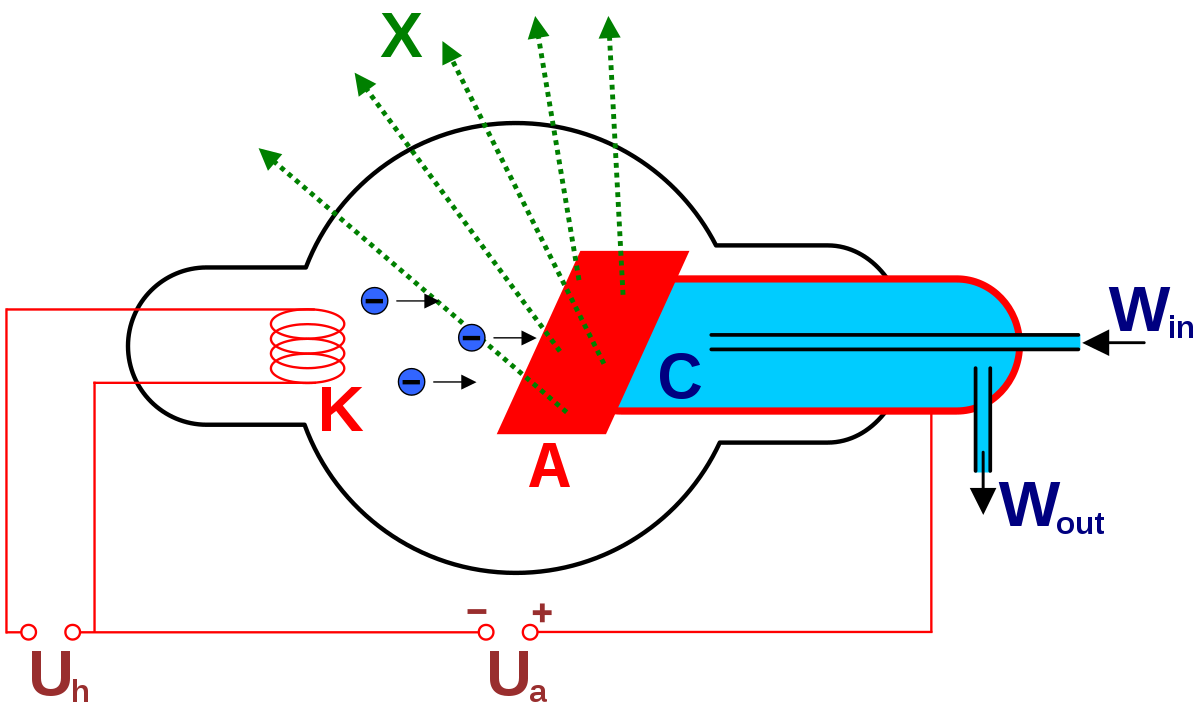
\includegraphics[width=0.45\textwidth]{Fig/tube-a-rayon-x.png} 
    \caption{Tube à rayons X}
    \label{fig:tube à rayons X}
\end{wrapfigure}
\vspace{1.5cm}
On applique une forte différence de potentiel (plusieurs dizaines de kV) 
entre la cathode et l'anode afin d'accélérer les électrons.
\textbf{Leur énergie cinétique $E_c = U e$ avec $U$ en Volt et $e$ en Coulomb ce qui donne des Joules.}
Lors de l'impact des électrons sur la  cible (AC), des rayons X sont émis.

\vspace{2cm}
\subsection{Spectre d'émission des rayons X}

\subsubsection{Le fond continu}

Il est émis par les électrons ralentis dans la cible lorsque qu'ils sont 
brusquement freinés dans le champ électrique (on dit alors qu'ils sont diffusés, voir figure \ref{fig:origine fond continu}). 
L'énergie $\frac{h\nu}{e}$ (en \qty{}{eV}) des rayons X ainsi produits étant au plus égale à l'énergie des 
électrons incidents ($E_{cin}$), avec $U$ étant la tension d'accélération en volt, on en déduit que:
$$\frac{hc}{\lambda e} \le U \quad \Longleftrightarrow \quad \lambda \ge \frac{hc}{eU}$$

Comme les électrons perdent inégalement leur énergie dans la matière de l'anticathode, 
le rayonnement X a un spectre continu de radiations au-delà d'un seuil de longueur d'onde, 
dont la valeur $\lambda_0$ est tout simplement égale à ($\frac{hc}{eU}$). 


L'allure de ce fond continu dépend de la tension d'accélération, comme l'indique la Figure \ref{fig:Spetre RX fond continu}.

\begin{figure}[ht]
    \centering
    \begin{subfigure}{0.48\textwidth}
        \centering
        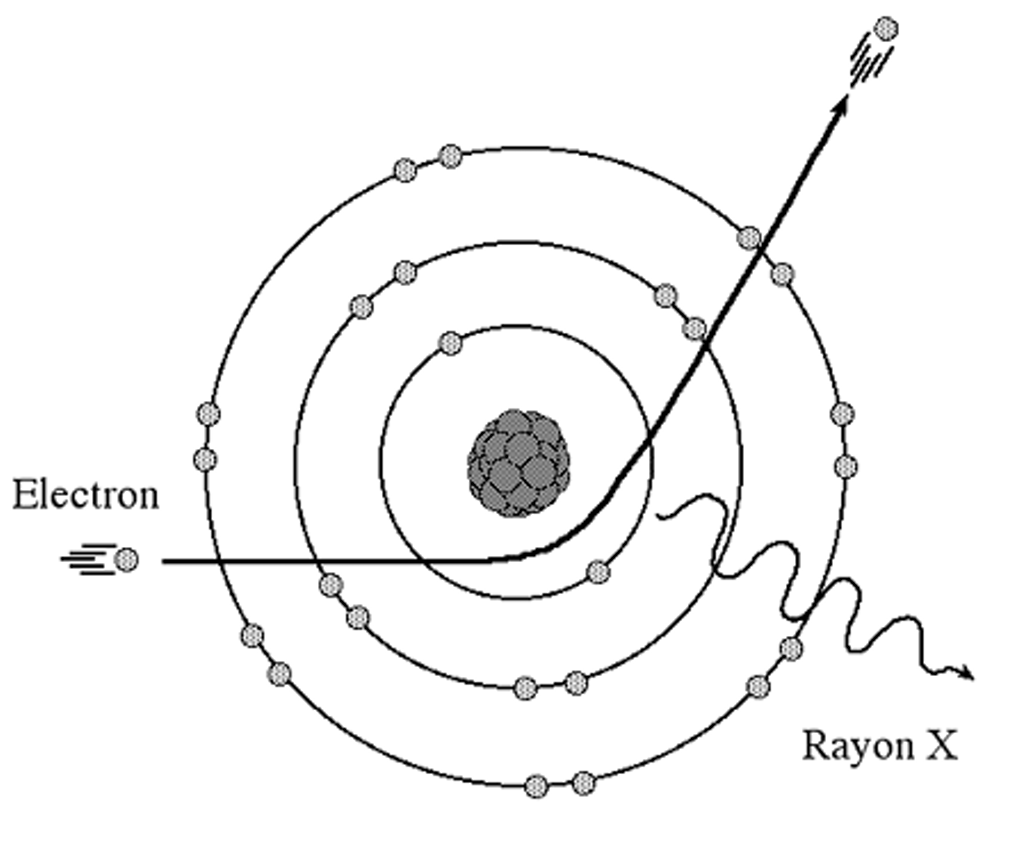
\includegraphics[width=0.9\linewidth]{Fig/origine-fond-continu.png}
        \caption{L'origine du fond continu}
        \label{fig:origine fond continu}
    \end{subfigure}
    \hfill\begin{subfigure}{0.48\textwidth}
        \centering
        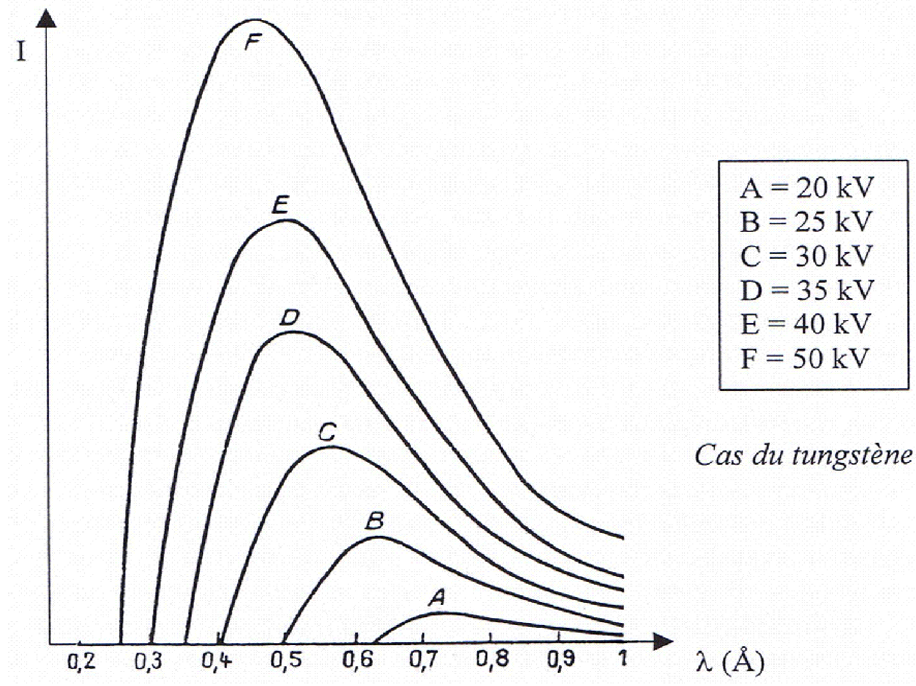
\includegraphics[width=0.9\linewidth]{Fig/Spectre-RX-fond-continu.png}
        \caption{Allure du fond continu en fonction de la tension accélératrice}
        \label{fig:Spetre RX fond continu}
    \end{subfigure}
\end{figure}

\newpage

\subsubsection{Le spectre de raies caractéristiques}
Les raies caractéristiques sont émises par les atomes constituant l'anticathode si la tension 
accélératrice est suffisante (sinon on a seulement un fond continu).
Le photon ou l'électron lancé sur l'anticathode ionise un électron de la couche $K$ (voir figure \ref{fig:origine des raies caractéristiques}). Le vide est alors comblé par un électron d'une couche supérieure $L$, $M$ \dots 
\, \textbf{C'est ce replacement d'électron au sein de l'anticathode qui est à l'origine de l'émission d'un photon d'énergie importante (rayonnement X).}
Les spectres de tout les éléments sont analogues: constitués de séries de raies 
nommées $K, L, M, $ \dots

Pour expliquer ces spectres, on introduit un nouveau nombre quantique noté $j$ qui modélise un \textbf{couplage spin-orbite} de l'électron (à la fois le moment cinétique autour du noyau et autour de lui même).
$$j=\left|l\pm \frac{1}{2}\right|$$

L'introduction de ce couplage spin-orbite permet d'interpréter la structure fine des 
spectres, car il introduit une perturbation de l'énergie du système. Cette perturbation dépend de 
la valeur de $j$ et est d'autant plus grande que le numéro atomique $Z$ de l'élément est élevé. 
Chaque niveau d'énergie, caractérisé par un couple de valeurs ($n, l$) est donc dédoublé 
(sauf pour les niveaux $ns$) en deux sous-niveaux d'énergie différente, notés $\bm{n}l_j$.

\textbf{Exemple:} \quad $l=2$ \quad $j=2\pm \frac{1}{2} \; \rightarrow \; \underbrace{j=\frac{5}{2}}$ ou $\underbrace{j=\frac{3}{2}}$

\hspace{5.8cm} $nd_{5/2}$ \hspace{0.7cm} $nd_{3/2}$


\begin{figure}[ht]
    \centering
    \begin{subfigure}{0.48\textwidth}
        \centering
        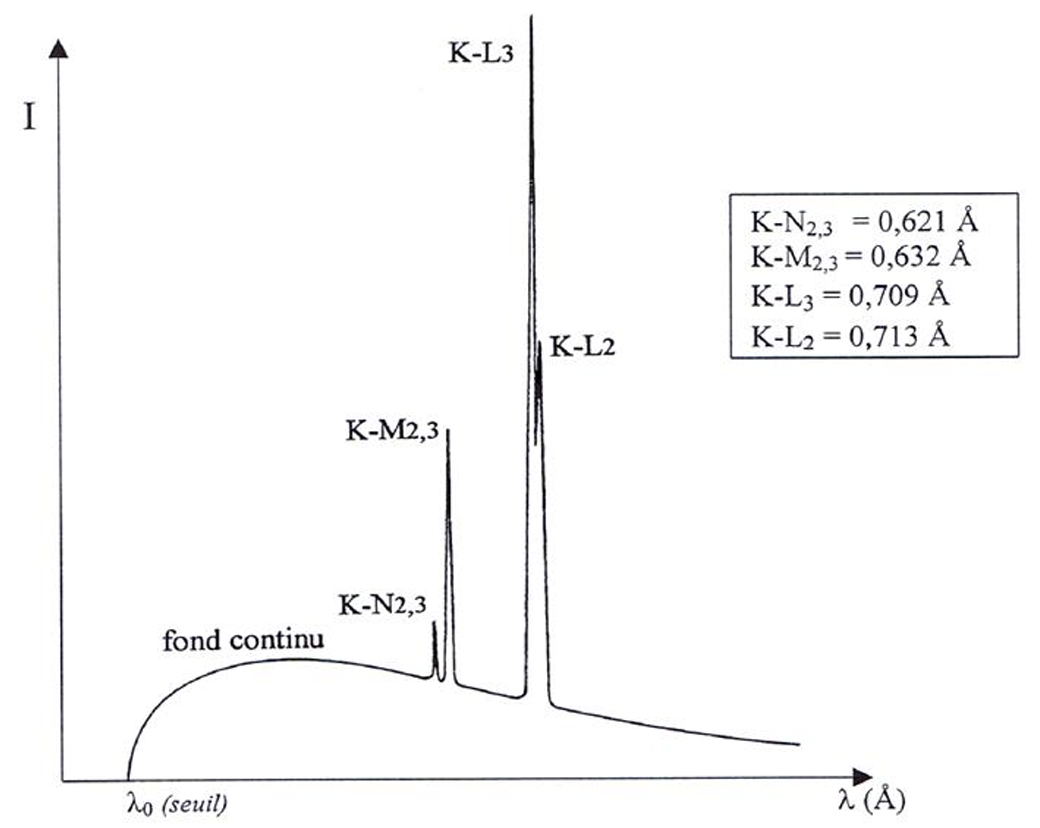
\includegraphics[width=0.9\linewidth]{Fig/Spectre-RX.png}
        \caption{Allure d'un Spectre RX}
        \label{fig:Spectre RX}
    \end{subfigure}
    \hfill\begin{subfigure}{0.48\textwidth}
        \centering
        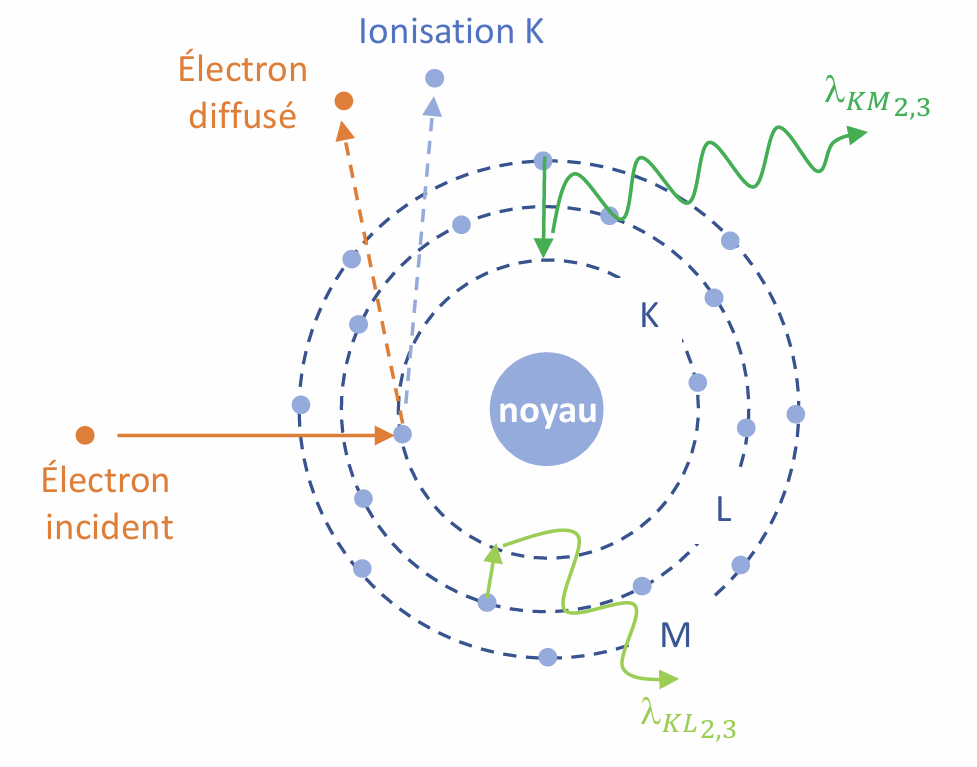
\includegraphics[width=0.9\linewidth]{Fig/origine-raies-rx.png}
        \caption{L'origine des raies caractéristiques}
        \label{fig:origine des raies caractéristiques}
    \end{subfigure}
\end{figure}


\subsubsection{Les règles de transitions}

\setlength{\intextsep}{0pt}
\begin{wrapfigure}{r}{0.45\textwidth}
    \centering
    \vspace{-1.5cm}
    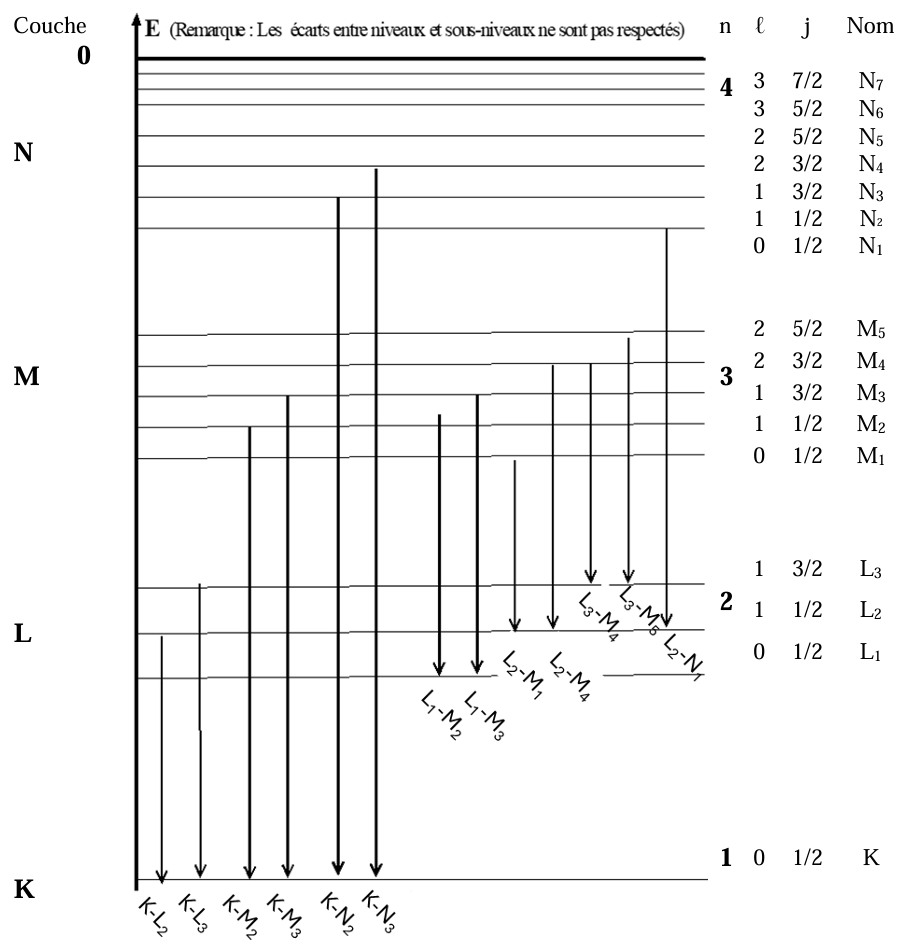
\includegraphics[width=0.45\textwidth]{Fig/Grotrian-RX.png} 
    \caption{Transitions possibles entre les différents niveaux}
    \label{fig:Transitions possibles}
\end{wrapfigure}
\vspace{5mm}
Comme le montre la figure \ref{fig:origine des raies caractéristiques}, 
les RX sont produit lorsqu'un électron d'une couche périphérique va vers la couche $K$ de l'anticathode. 
Ces transitions sont identifiées par deux lettres correspondant aux niveaux d'arrivée puis de départ de l'électron. 
Les indices 1, 2, 3, \dots \,caractérisent les sous-niveaux. 
Par exemple, la raie $K\text{-}L_3$ correspond à une transition entre $L_3\, (2p_{3/2})$ et $K\, (1s_{1/2})$. 

Les propriétés de l'électron (en particulier son moment cinétique de spin) font que seules seront permises 
les transitions pour lesquelles (voir aussi figure \ref{fig:Transitions possibles}):
$$\boxed{\Delta l = \pm 1 \quad et \quad \Delta j = \left\{0, \pm 1\right\}}$$  


\newpage
\clearpage

\subsection{Loi de Moseley pour les rayons X}

Moseley (1887-1915) constate que la fréquence $\nu$ d'une des raies de chacun des 
spectres étudiés (par exemple $K$-$L2$) était liée au numéro atomique $Z$ de cet élément par 
la relation:
$$\sqrt{\nu}=a(Z-b)=AZ+B$$

\begin{figure}[ht]
    \centering
    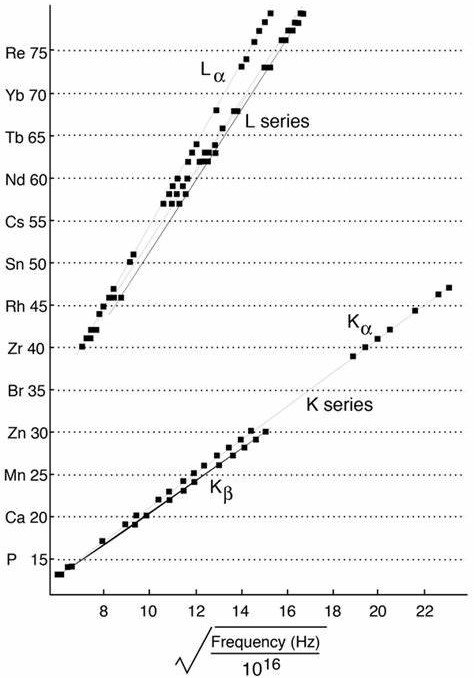
\includegraphics[width=0.5\textwidth]{Fig/Moseley.jpg}
    \caption{Tracé expérimental de Moseley}
    \label{fig:Moseley}
\end{figure}


\newpage
\subsection*{Exercice d'application: Loi de Moseley et Spectre RX}

\vspace{5mm}
\begin{tabular}{|c|c|c|c|c|c|c|c|}
    \hline
    \textbf{Elément} & \textbf{V} & \textbf{Cr} & \textbf{Mn} & \textbf{Fe} & \textbf{Co} & \textbf{Ni} & \textbf{Au} \\ \hline
    \textbf{Z} & 23 & 24 & 25 & 26 & 27 & 28 & ? \\ \hline
    $\bm{E_{K(eV)}}$ & -5465.0 & ? & -6540.0 & -7114.2 & -7711.4 & -8332.8 & -80724 \\ \hline
    $\bm{\Delta E_{K\text{-}L_{2,3}(eV)}}$ & -4950.1 & -5412.5 & -5895.5 & -6398.3 & -6923.5 & ? & -68201 \\ \hline
    $\bm{\Delta E_{K\text{-}M_{2,3}(eV)}}$ & -5429.1 & -5947.2 & -6492.1 & -7057.5 & -7649.6 & -8261.2 & -77845 \\ \hline
\end{tabular}
\vspace{5mm}
\begin{enumerate}
    \item Calculer les valeurs d'énergie manquantes pour le Chrome et le Nickel. Calculer le numéro atomique $Z$ de l'or et vérifiez sa validité avec le tableau périodique. Commentez.
\end{enumerate}

\vspace{5cm}

\noindent\textbf{Réponse:}  \vspace{3mm}

\textbf{1.} \quad On utilise la loi de Moseley (les éléments sont dans la même période, la loi est valable): 
$$\left\{ \begin{aligned}
    \sqrt{-E_{K_{(V)}}} &= AZ_{(V)} + B \quad &(L1) \\
    \sqrt{-E_{K_{(Mn)}}} &= AZ_{(Mn)} + B \quad &(L2) \\
    \sqrt{-E_{K_{(Cr)}}} &= AZ_{(Cr)} + B \quad &(L3) \\
\end{aligned} \right. $$
Pour exprimer $E_{K_{(Cr)}}$ sans calculer les constantes $A$ et $B$, on exprime $A$ en l'isolant dans $(L1)-(L2)$ et on fait de même avec $(L1)-(L3)$:
$$ A = \frac{\sqrt{-E_{K_{(V)}}} - \sqrt{-E_{K_{(Mn)}}}}{Z_{(V)} - Z_{(Mn)}} = \frac{\sqrt{-E_{K_{(V)}}} - \sqrt{-E_{K_{(Cr)}}}}{Z_{(V)} - Z_{(Cr)}} $$
$$ \Longleftrightarrow \quad -\sqrt{-E_{K_{(Cr)}}} = \frac{(Z_{(V)} - Z_{(Cr)}) \left( \sqrt{-E_{K_{(V)}}} - \sqrt{-E_{K_{(Mn)}}}\right)}{Z_{(V)} - Z_{(Mn)}} - \sqrt{-E_{K_{(V)}}}$$
$$ \Longleftrightarrow \quad E_{K_{(Cr)}} = -\left(\sqrt{-E_{K_{(V)}}} - \frac{(Z_{(V)} - Z_{(Cr)}) \left( \sqrt{-E_{K_{(V)}}} - \sqrt{-E_{K_{(Mn)}}}\right)}{Z_{(V)} - Z_{(Mn)}}\right)^2$$
$$ \text{\underline{AN:}} \quad E_{K_{(Cr)}} = -\left(\sqrt{5465} - \frac{(23-24) \left( \sqrt{5465} - \sqrt{6540}\right)}{23-25}\right)^2 = \qty{-5990.4}{eV}$$
On fait de même pour $\Delta E_{K\text{-}L_{2,3}(Ni)}$ avec les éléments Co et Fe et on obtient $\Delta E_{K\text{-}L_{2,3}(Ni)} = \qty{-7469.4}{eV}$

Si on faisait de même pour le numéro atomique de l'or, on trouverait $Z_{(Au)} = 83.5$. En effet, dans ce cas la loi de Moseley ne s'applique pas car l'or à un numéro atomique bien supérieur (pas dans la même période !).



\subsection{Atténuation des rayons X}

Pour atténuer l'intensité d'un rayon X, on peut intercaller un filtre qui atténuera certaines longueurs d'ondes. 
Ce phénomène d'atténuation sélective est notemment utilisé en radiographie.

Les photons qui arrivent sur le filtre interagissent alors avec les atomes par effet photoélectrique et diffusion.
\begin{itemize}[label=$\ast$]
    \item \textbf{Interaction photoélectrique} : photon absorbé et électron arraché : $E_{\text{inscident}} = E_{\text{électron}} + E_c$.
    Lors de la réorganisation des couches, est émis un rayonnement de fluorescence caractéristique du filtre.
    \item \textbf{Diffusion} : photon absorbé, un électron absorbe une partie de l'énergie et est éjecté, et le reste de l'énergie contribue à l'émission d'un photon secondaire.
\end{itemize}

\subsubsection{Loi d'atténuation exponentielle: loi de Beer-Lambert}

\setlength{\intextsep}{0pt}
\begin{wrapfigure}[5]{r}{0.5\textwidth} % the [6] means that only 6 lines will be wrapped left to the fig
    \centering
    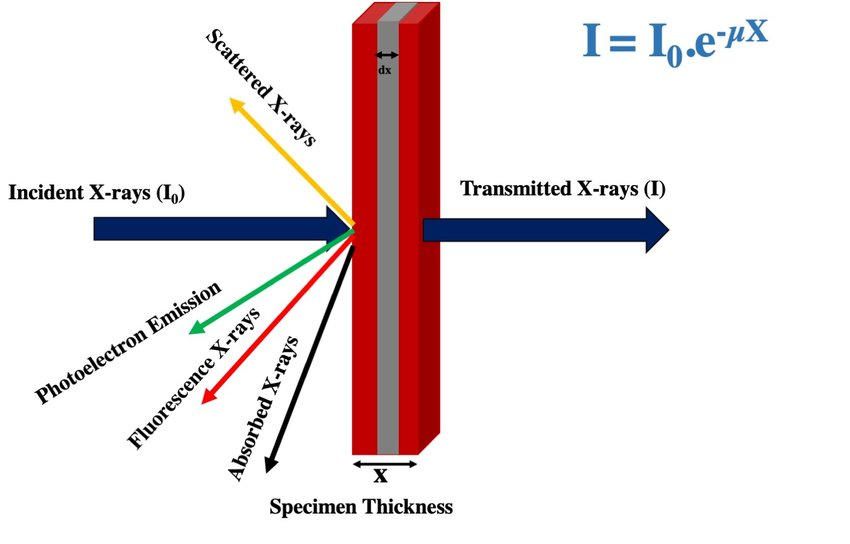
\includegraphics[width=0.5\textwidth]{Fig/Beer-Lambert-law-X-rays-to-solid-matter-interaction.png} 
    \caption{Intensité d'une raie d'après la loi de Beer-Lambert}
    \label{fig:Beer Lambert}
\end{wrapfigure}


$I_0$ est l'intensité de la raie intiale et $I$ l'intensité de la raie après filtre de largeur $x$.
\vspace{1cm}
{\Large$$I=I_0 \exp{(-\mu x)}$$} 

\vspace{3.5cm}

\subsubsection{Conditions de monochromatisation d'un signal}

Il est important de pouvoir monochromatiser un signal (c'est à dire ne garder qu'une seule longueur d'onde) afin d'obtenir des résultats précis pour une mesure. 
Il faut donc \textbf{laisser passer la raie la plus intense} ($K\text{-}L$) \textbf{et absorber la raie la moins intense} ($K\text{-}M$) qui est la plus énergétique.
Le filtre permettant cette monochromatisation doit respecter ces conditions:
\begin{itemize}[label=$\ast$]
    \item  $\lambda_{K\text{-}M (AC)} < \lambda_{K (filtre)} < \lambda_{K\text{-}L (AC)} \quad$ ou $E_{K\text{-}M (AC)} > E_{K (filtre)} > E_{K\text{-}L (AC)}$
    \item Pour un métal de numéro atomique $Z$, une règle générale dit que le filtre doit être un métal de numéro atomique $Z-1$ pour assurer une bonne monochromatisation.
\end{itemize}

\vspace{5mm}
\begin{figure}[h]
    \centering
    \begin{subfigure}{0.48\textwidth}
        \centering
        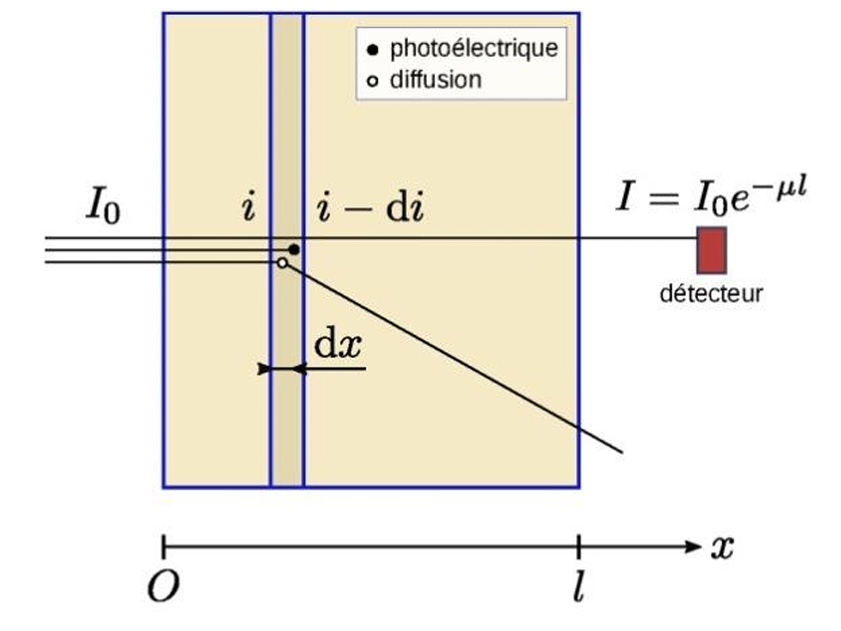
\includegraphics[width=0.8\linewidth]{Fig/filtre-rx.png}
        \caption{Atténuation d'un faisceau de photons}
        \label{fig:atténuation photons}
    \end{subfigure}
    \hfill\begin{subfigure}{0.48\textwidth}
        \centering
        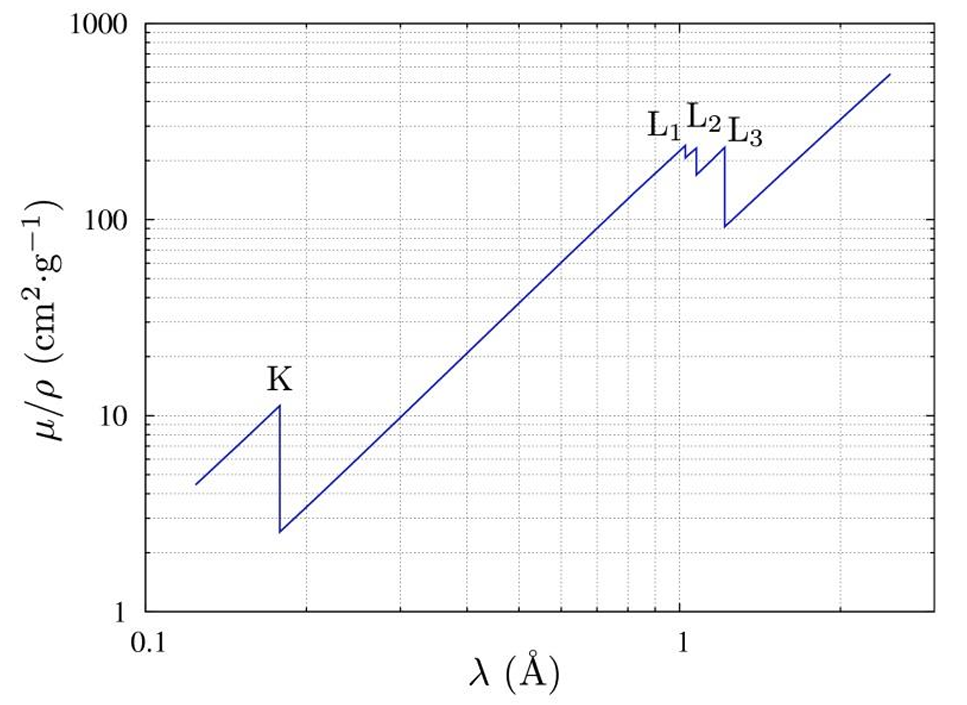
\includegraphics[width=0.7\linewidth]{Fig/coef_absorption.png}
        \caption{Coefficient d'atténuation massique du tungstène (W) en fonction de la longueur d'onde (source : NIST Standard Reference Database). }
        \label{fig:coef absoption}
    \end{subfigure}
\end{figure}




\section{Liaison Covalente}\label{sec:Liaison covalente}
\textbf{Les atomes se rapprochent de manière à minimiser l'énergie totale.}
Les atomes s'attirent mutuellement (électrons de A avec noyau de B) mais, quand ils se rapprochent trop, il y a une répulsion entre le noyau de A avec noyau de B.


\subsection{Théorie de Lewis}

\noindent\textbf{Électrons de valence:} Electrons du plus grand nombre quantique principal $n$ et d'une sous-couche avec $n$ inférieur non totalement remplie.

\noindent\textbf{Liaison covalente:} Mise en commun de deux élections pour former une doublet de liaison:
\begin{itemize}[label=$\ast$]
    \item \textbf{Covalence typique:} Chacun des deux atomes fournit un électron.
    \item \textbf{Covalence dative ou coordinence:} Un atome fournit un doublet déjà constitué, l'autre le reçoit dans une case vide de sa couche externe.
    On a alors des charges formelles $^+$ pour le donneur et $^-$ pour le receveur.
\end{itemize}

\noindent\textbf{Longueur des liaisons:} Si la liaison est double, la liaison sera plus courte (atomes plus rapprochés).

\noindent\textbf{Règles du duet et de l'octet:} L'Hydrogène sera entouré de deux électrons (duet), puis de 8 électrons pour C, N, O, F.
Pour $n \ge 3$, chaque électron de valence peut former un doublet (extension de la règle de l'octet car possibilité d'absorption par la couche $d$).

\noindent\textbf{Théorie de la mésomérie:} Les liaisons double/triples peuvent se délocaliser, ce qui donne des forumules mésomères.
Mais les formules mésomères n'ont pas de réalité physique, on définie alors ce qu'est un hybride de résonance.
Les formules mésomères les plus probables sont alors celles qui minimisent la séparation des charges et qui attribuent les charges formelles négatives aux atomes les plus électronégatifs.

\noindent\textbf{Valence :} Le nombre de liaisons covalentes qu'un élément établit (correspond en général au nombre d'électrons non appariés, en désappariant au maximum les cases quantiques pleines).\\
Voir le tableau \ref{tab:Valence}. 

\vspace{5mm}\begin{table}[h]
    \centering
    {\setlength{\extrarowheight}{5pt}%
    \begin{tabular}{|c|c|c|c|c|}
        \hline
        \textbf{Atome} & \makecell{\textbf{Configuration} \\ \textbf{électronique}} & \makecell{\textbf{Représentation cases} \\ \textbf{quantiques}} & \makecell{\textbf{Représentation de} \\ \textbf{Lewis nfondamentale}} & \makecell{\textbf{Représentation de} \\ \textbf{Lewis usuelle}} \\ \hline
        $_1H$ & $\bm{1s^1}$ & \makecell{ \\ \electron{1s}{\haut} \\ \\ } \vspace{-2mm} &  {\large\charge{0=\.}{H}} & {\large\charge{0=\.}{H}} \\ \hline
        $_7N$ & $1s^1\bm{2s^22p^3}$ & \makecell{ \\ \electron{2s}{\updwn} \quad \electron{2p}{\haut \ \haut \ \haut} \\ \\ }\vspace{-2mm}  &  {\large \charge{270=\., 0=\., 180=\., 90=\|}{N}} & {\large \charge{270=\., 0=\., 180=\., 90=\:}{N}} \\ \hline
        $_9O$ & $1s^1\bm{2s^22p^4}$ & \makecell{ \\ \electron{2s}{\updwn} \quad  \electron{2p}{\updwn \ \haut \ \haut} \\ \\ }\vspace{-2mm}  &  {\large \charge{270=\., 0=\., 180=\|, 90=\|}{O}} & {\large \charge{270=\., 0=\., 180=\:, 90=\:}{O}} \\ \hline
        $_{17}Cl$ & $1s^12s^22p^6\bm{3s^23p^5}$ & \makecell{ \\ \electron{3s}{\updwn} \quad \electron{3p}{\updwn \ \updwn \ \haut} \\  } & {\large \charge{270=\|, 0=\., 180=\|, 90=\|}{Cl}} & {\large \charge{270=\:, 0=\., 180=\:, 90=\:}{Cl}} \\ \hline
    \end{tabular}}
    \caption{Valence de différents atomes}
    \label{tab:Valence}
\end{table}

\subsubsection{Polarisation de la liaison covalente}

L'atome le plus électronégatif attire les électrons vers lui : liaison polarisée pour $0,4 < \Delta\chi < 2$.\\
Moment dipolaire de l'atome le plus électronégatif ($\chi$ supérieur, noté $\delta^-$) vers le moins électronégatif :\\
$\mu = q \times d$ où $d$ est la longueur de la liaison et $q = \delta \times e$ ($\delta$ pourcentage d'ionicité, dépend de $\Delta \chi$).\\
Molécule apolaire : aucune polarité individuelle.
Molécule non polaire : somme des moments dipolaires nuls.


\newpage

\subsection{Géométrie des molécules: méthode VSEPR}

\vspace{5mm}

\textbf{VSEPR:} Valence Shell Electron Pair Repulsion.

\vspace{5mm}
\begin{center}
    \begin{tabular}{|c|c|c|c|c|}
        \hline
        \textbf{Formule} $\bm{AX_nE_p}$ & \textbf{Géométrie} & \textbf{Exemple} & \textbf{Représentation spatiale} & \textbf{Angle} \\ \hline
        $\bm{AX_2}$ & Linéaire & \ce{CO2} & \makecell{ \\
        \chemfig{C(-[:0]O)(-[:180]O)} \\ \\ }\vspace{-2mm} & \ang{180} \\ \hline
        $\bm{AX_3}$ & Trigonale plane & \ce{AlCl3} & 
        \makecell{ \\ \chemfig{Al(-[:0, .9]Cl)(-[:120, .9]Cl)(-[:-120, .9]Cl)} \\ \\ }\vspace{-2mm}  & \ang{120} \\ \hline
        $\bm{AX_2E_1}$ & Coudée en V & \ce{SO2} & 
        \makecell{\orbital[color=gray, half]{p} \\ \vspace{-2mm}\chemfig{O-[::+50, .8]S-[::-100, .8]O} \\ \\ } & $<\ang{120}$ \\ \hline
        $\bm{AX_4}$ & Tétraédrique & \ce{CH4} & 
        \makecell{ \\ \chemfig{C(-[:90, .9]H)(<[:-30, .9]H)(-[:-150, .9]H)(<:H)} \\ \\  }\vspace{-1mm} & \ang{109.5} \\ \hline
        $\bm{AX_3E_1}$ & \makecell{Pyramidale à \\ base trigonale} & \ce{NH3} & 
        \makecell{\, \orbital[color=gray, half]{p} \\ \chemfig{N(<[:-160]H)(-[:-40, 1.1]H)(<:[:-130]H)} \\ \\ } \vspace{-2mm} & $<\ang{109.5}$ \\ \hline
        $\bm{AX_2E_2}$ & Coudée & \ce{H2O} & 
        \hspace{-8mm}\makecell{\raisebox{2mm}{\orbital[angle=135, color=gray, half]{p} \, \orbital[angle=35, color=gray, half]{p}} \hspace{-1.7cm}\chemfig{O(<[:-110, .9]H)(<:[:-70, .9]H)} \\ \\ } \vspace{-2mm} & $<\ang{109.5}$ \\ \hline
        $\bm{AX_5}$ & \makecell{Bipyramidale \\ trigonale} & \ce{PCl5} & 
        \makecell{ \\ \chemfig{P(-[:90, .9]Cl)(-[:180, .9]Cl)(-[:-90, .9]Cl)(<[:-30, .8]Cl)(<:[:30, .8]Cl)} \\ \\ }\vspace{-2mm} & \makecell{\ang{120} horizontal \\ \ang{90} vertical} \\ \hline
        $\bm{AX_6}$ & Octaédrique & \ce{SF6} & 
        \makecell{ \\ \chemfig{S(-[:90, .9]F)(-[:-90, .9]F)(<:[:30, .8]F)(<[:-30, .8]F)(<[:-150, .8]F)(<:[:150, .8]F)} \\ \\ }\vspace{-2mm}  & \ang{90} \\ \hline
        $\bm{AX_4E_2}$ & Plan carré & \ce{XeF4} & 
        \makecell{\raisebox{3mm}{\orbital[color=gray, half]{p}} \hspace{-1.75cm}\chemfig{Xe(<:[:30, .9]F)(<[:-30, .9]F)(<[:-150, .9]F)(<:[:150, .9]F)} \hspace{-1.8cm}\raisebox{-1mm}{\orbital[angle=270, color=gray, half]{p}} \\ } & \ang{90} \\ \hline
    \end{tabular}
\end{center}

\clearpage

\subsection{Hybridation: modèle ondulatoire de la liaison covalente}





\section{Oxydoréduction}\label{sec:oxydoréduction}

\subsection{Rappels Oxydoréduction}\label{subsec:rappels-oxydoreduction}
\ce{Ox + ne^- <=> Red}

\subsection{Degré d'oxydation}\label{subsec:degre-d'oxydation}

On calcule le nombre d'électrons après une \textbf{ionisation fictive} :
\begin{itemize}[label=$\ast$]
    \item Liaisons polarisées : L'atome le plus électronégatif prend tous les électrons de la liaison.
    \item Liaison non polarisée : Chaque atome garde ses électrons (moitié-moitié).
\end{itemize}

$$\text{Nombre d'oxydation} = \text{Électrons de valence} - \text{Électrons après ionisation fictive}$$

\vspace{5mm}
\noindent\textbf{Quelques infos importantes:}
\begin{itemize}[label=$\ast$]
    \item Pour une molécule formée d'atome identiques, $n.o. = 0$.
    \item L'Hydrogène $H$ aura souvent $n.o. = \mathrm{I}$.
    \item Le Fluor $F$ aura toujours $-\mathrm{I}$ sauf s'il est liée à lui-même.
    \item l'Oxygène $O$ aura toujours $-\mathrm{II}$, sauf s'il est lié au Fluor ou à lui même.
    \item Dans une rédox, l'oxydant a le $n.o.$ le plus élevé.
    \item Pour un ion, $n.o. = \text{charge de l'ion}$
    \item Le nombre d'oxydation d'un atome $X$ donne le nombre d'électrons échangés par atome $X$.
    \item La somme des $n.o.$ dans une molécule est nulle (ou vaut la charge de l'ion polyatomique).
\end{itemize}


\section{Modèle du cristal parfait}\label{ch:modele-du-cristal-parfait}


\subsection{L'architecture du cristal}\label{sec:l'architecture-du-cristal}

\subsubsection{Vocabulaire}\label{subsec:vocabulaire}

\noindent\textbf{Motif :} unité élémentaire répétée dans le cristal, composé de $\frac{N_X}{m}$ molécules ($m$: multiplicité de la maille).

\noindent\textbf{Réseau :} ensemble de points répétés à l'infini, où chaque point est un motif. Son origine n'a pas d'importance.
Le réseau peut être défini par trois vecteurs de base partant d'un point arbitraire.

\noindent\textbf{Noeud :} point obtenu par combinaison linéaire des vecteurs de la base du réseau.

\noindent\textbf{Maille :} parallélépipède construit sur un vecteur $\vec V$, contenant $N_X$ molécules.
Les longueurs $a$, $b$, $c$ et les angles $\alpha$, $\beta$ et $\gamma$ sont les paramètres de la maille.

\noindent\textbf{Maille simple} ne contient des noeuds qu'en ses huit sommets : ne contient qu'un noeud en moyenne.

\noindent\textbf{Maille multiple} contient en moyenne plus d'un noeud : on parle de multiplicité $m$.
Une maille multiple aura un volume $m$ fois plus grand que celui de la maille simple correspondante.


\subsubsection{Les sept systèmes cristallins et les 14 réseaux de Bravais}\label{subsec:les-sept-systemes-cristallins-et-les-14-reseaux-de-bravais}

On classe les parallélépipèdes constitutifs du réseau de translation tri-périodique en sept systèmes cristallins.
Bravais a démontré que pour certains systèmes, on peut avoir une maille multiple.
On a donc en plus des mailles simples, des mailles à intérieur centrée, à bases centrées et à toutes faces centrées.
Tout cela définit les modes de réseau.
Il y a 14 réseaux de Bravais représentés figure \ref{fig:bravais}.

\vspace{0.4cm}
\subsubsection{Éléments et opérations de symétrie}\label{subsec:elements-et-operations-de-symetrie}

\begin{wrapfigure}[5]{r}{0.3\textwidth}
    \raggedright
    \vspace{-1.5cm}
    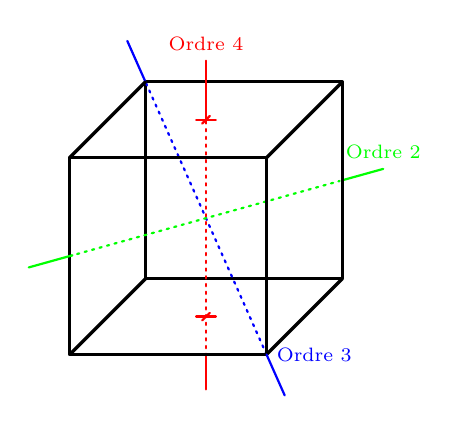
\begin{tikzpicture}[scale=2.5, line join=round, line cap=round]

        % Définir les sommets d'un cube
        \coordinate (A) at (0, 0, 0);
        \coordinate (B) at (1, 0, 0);
        \coordinate (C) at (1, 1, 0);
        \coordinate (D) at (0, 1, 0);
        \coordinate (E) at (0, 0, 1);
        \coordinate (F) at (1, 0, 1);
        \coordinate (G) at (1, 1, 1);
        \coordinate (H) at (0, 1, 1);
        
        \draw[green, thick] (1, 0.5, 0) -- (1.15, 0.5, -0.15) node[above, green] {\scriptsize Ordre 2};
    
        \draw[black, very thick] (A) -- (B) -- (C) -- (D) -- cycle; % Face de derriere
        
        % Axe d'ordre 4 (centre de deux faces opposées)
        \draw[red, thick, dotted] (0.5, -0.2, 0.5) -- (0.5, 1, 0.5);
        \draw[red, thick] (0.5, -0.37, 0.5) -- (0.5, -0.2, 0.5);
        \draw[red, thick] (0.5, 1, 0.5) -- (0.5, 1.3, 0.5) node[above, red] {\scriptsize Ordre 4};
        \draw[red, thick] (0.5, 0, 0.45) -- (0.5, 0, 0.55); % cross
        \draw[red, thick] (0.45, 0, 0.5) -- (0.55, 0, 0.5); % cross
        \draw[red, thick] (0.5, 1, 0.45) -- (0.5, 1, 0.55); % cross
        \draw[red, thick] (0.45, 1, 0.5) -- (0.55, 1, 0.5); % cross
    
        % Axe d'ordre 3 (grande diagonal)
        \draw[blue, thick, dotted] (1, 0, 1) -- (0, 1, 0);
        \draw[blue, thick] (0, 1, 0) -- (-0.15, 1.15, -0.15);
    
        % Axe d'ordre 2 (centre de deux aretes opposées)
        \draw[green, thick, dotted] (0, 0.5, 1) -- (0.99, 0.5, 0.01);
       
    
        % Tracer les arêtes du cube
        \draw[black, very thick] (E) -- (F) -- (G) -- (H) -- cycle; % Face supérieure
    
        \draw[green, thick] (0.01, 0.5, 0.99) -- (-0.15, 0.5, 1.15);
    
        \draw[black, very thick] (A) -- (E); % Arêtes verticales
        \draw[black, very thick] (B) -- (F);
        \draw[black, very thick] (C) -- (G);
        \draw[black, very thick] (D) -- (H);
    
        \draw[blue, thick] (1.15, -0.15, 1.15) -- (1, 0, 1) node[right, blue] {\scriptsize Ordre 3};
    \end{tikzpicture}
\end{wrapfigure}

\noindent La symétrie explique pourquoi on a que 14 réseaux de Bravais et non $28$ ($7$ systèmes $\times$ $4$ modes de réseaux).\\
Un axe de rotation peut être $A_2$, $A_3$, $A_4$ ou $A_6$ (ordre $n \rightarrow (\frac{2\pi}{n})^{\circ}$ de rotation)

\noindent Les axes de symétrie du cube sont : $3A_4$, $4A_3$ et $6A_2$ (Les axes $A_4$ n'existent que s'il y a des faces carrées).

\vspace{0.4cm}

\subsubsection{Sites interstitiels dans un réseau cubique toutes faces centrées}\label{subsec:sites-intersticiels-dans-un-reseau-cubique-toutes-faces-centrees}

La maille cubique contient 8 sites tétraédriques en propre (formé à partir des sommets), et 4 sites octaédriques (un quart par arête).\\
Les sites tétraédriques se trouvent à une distance égale à $\frac{a\sqrt{3}}{4} = a\sqrt{3} \times \frac{1}{3} \times \frac{3}{4}$ de chaque sommet du cube. $a$ étant le paramètre de maille.\\
Ces sites peuvent accueillir des atomes, ions ou molécules en leur centre.

\vspace{10mm}
\begin{figure}[h]
    \centering
    \begin{subfigure}{0.48\textwidth}
        \centering
        \begin{tikzpicture}[scale=3.5, x={(1.1,0)}, y={(0,1.2)}, z={(0, 0, 1.2)}, line join=round, line cap=round]

            % Cube edges
            \draw[gray, very thick] (0,0,0) -- (1,0,0) -- (1,1,0) -- (0,1,0) -- cycle; % face du fond
    
            % Vertices of the cube (background)
            \foreach \x/\y/\z in {0/0/0, 1/0/0, 1/1/0, 0/1/0, 0.5/0.5/0, 0/0.5/0.5, 0.5/0/0.5} {
                \fill[black] (\x,\y,\z) circle (0.03);
            }
    
           
            \fill[darkgreen!70!green] (0.5,0.5,0.5) circle (0.04);
           
    
            % Octahedral site (green) (background)
            \foreach \x/\y/\z in {0.5/0/0, 0/0.5/0} {
                \fill[darkgreen] (\x, \y, \z) circle (0.03);
            }
    
            % aretes sites octa
            \draw[green, thick, dotted][dash pattern=on 1mm off 0.8mm] (0.5,0.5,0) -- (0.5,0,0.5); % face de derriere
            \draw[green, thick, dotted][dash pattern=on 1mm off 0.8mm] (0.5,0.5,0) -- (0.5,1,0.5);
            \draw[green, thick, dotted][dash pattern=on 1mm off 0.8mm] (0.5,0.5,0) -- (0,0.5,0.5);
            \draw[green, thick, dotted][dash pattern=on 1mm off 0.8mm] (0.5,0.5,0) -- (1,0.5,0.5);
    
            \draw[green, thick] (0.5,1,0.5) -- (1,0.5,0.5); % entre noeud faces
            \draw[green, thick] (1,0.5,0.5) -- (0.5,0,0.5); % entre noeud faces
            \draw[green, thick] (0.5,0,0.5) -- (0,0.5,0.5); % entre noeud faces
            \draw[green, thick] (0.5,1,0.5) -- (0,0.5,0.5); % entre noeud faces
            
            % cube top face verteses and right face
            \fill[black] (0.5,1,0.5) circle (0.03);
            \fill[black] (1,0.5,0.5) circle (0.03);
            
            % entre noeud face avant
            \draw[green, thick] (0.5,0.5,1) -- (0.5,0,0.5); % face de devant
            \draw[green, thick] (0.5,0.5,1) -- (0.5,1,0.5);
            \draw[green, thick] (0.5,0.5,1) -- (0,0.5,0.5);
            \draw[green, thick] (0.5,0.5,1) -- (1,0.5,0.5);
            
            % cube aretes
            \draw[gray, very thick] (0,0,0) -- (0,0,1); 
            \draw[gray, very thick] (1,0,0) -- (1,0,1);
            \draw[gray, very thick] (1,1,0) -- (1,1,1);
            \draw[gray, very thick] (0,1,0) -- (0,1,1);
            \draw[gray, very thick] (0,0,1) -- (1,0,1) -- (1,1,1) -- (0,1,1) -- cycle; % face avant
    
             % Octahedral site (green)
             \foreach \x/\y/\z in {0.5/1/0, 0.5/0/1, 0.5/1/1, 1/0.5/0, 0/0.5/1, 1/0.5/1, 0/0/0.5, 1/0/0.5, 0/1/0.5, 1/1/0.5} {
                \fill[darkgreen!70!green] (\x, \y, \z) circle (0.03);
            }
    
            % Vertices of the cube (foreground)
            \foreach \x/\y/\z in {0/0/1, 1/0/1, 1/1/1, 0/1/1, 0.5/0.5/1} {
                \fill[black] (\x,\y,\z) circle (0.03);
            }
    
        \end{tikzpicture}
        \caption{Sites Octaédriques dans une maille cubique faces centrées (1 seul octaèdre représenté)}
        \label{fig:cfc_sites}
    \end{subfigure}
    \hfill\begin{subfigure}{0.48\textwidth}
        \centering
        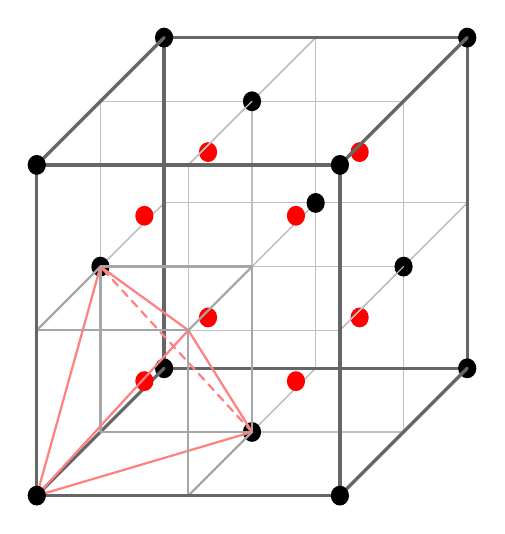
\begin{tikzpicture}[scale=3.5, x={(1.1,0)}, y={(0,1.2)}, z={(0, 0, 1.2)}, line join=round, line cap=round]

            % site tetra arriere
            \foreach \x/\y/\z in {0.25/0.25/0.25, 0.25/0.75/0.25, 0.75/0.25/0.25, 0.75/0.75/0.25} {
                \fill[red] (\x,\y,\z) circle (0.03); % Tetrahedral sites
            }
    
            % Edges of the small cubes (a/2)
            \foreach \x in {0, 0.5, 1} {
                \foreach \y in {0, 0.5, 1} {
                    \foreach \z in {0, 0.5, 1} {
                        % Draw edges of each small cube
                        \draw[lightgray, thin] (\x,\y,0) -- (\x,\y,1); % vertical edges
                        \draw[lightgray, thin] (\x,0,\z) -- (\x,1,\z); % edges parallel to y-axis
                        \draw[lightgray, thin] (0,\y,\z) -- (1,\y,\z); % edges parallel to x-axis
                    }
                }
            }
    
            % Cube edges (main cube)
            \draw[black!60, very thick] (0,0,0) -- (1,0,0) -- (1,1,0) -- (0,1,0) -- cycle; % face arriere
             % Vertices of the main cube (face arriere)
             \foreach \x/\y/\z in {0/0/0, 1/0/0, 1/1/0, 0/1/0, 0.5/0.5/0, 0/0.5/0.5, 0.5/0/0.5} {
                \fill[black] (\x,\y,\z) circle (0.03);
            }
            % cube edge
            \draw[black!60, very thick] (0,0,0) -- (0,0,1);
            \draw[black!60, very thick] (1,0,0) -- (1,0,1);
            \draw[black!60, very thick] (1,1,0) -- (1,1,1);
            \draw[black!60, very thick] (0,1,0) -- (0,1,1);
    
            % site tetra avant
            \foreach \x/\y/\z in {0.25/0.25/0.75, 0.25/0.75/0.75, 0.75/0.25/0.75, 0.75/0.75/0.75} {
                \fill[red] (\x,\y,\z) circle (0.03);
            }
            %cube ou ya le tetraedre
            \draw[gray!70, thick] (0,0,0.5) -- (0.5,0,0.5) -- (0.5,0.5,0.5) -- (0,0.5,0.5) -- cycle; % face arriere
    
            % tetraedre side
            \draw[red!50, thick] (0,0,1) -- (0.5,0,0.5);
            \draw[red!50, thick] (0,0,1) -- (0,0.5,0.5);
            \draw[red!50, thick] (0,0,1) -- (0.5,0.5,1);
            \draw[red!50, thick] (0,0.5,0.5) -- (0.5,0.5,1);
            \draw[red!50, thick] (0.5,0,0.5) -- (0.5,0.5,1);
            \draw[red!50, thick, dotted][dash pattern=on 1mm off 0.8mm] (0.5,0,0.5) -- (0,0.5,0.5);
    
            % petit cube ou ya le tatraedre
            \draw[gray!70, thick] (0,0,1) -- (0.5,0,1) -- (0.5,0.5,1) -- (0,0.5,1) -- cycle; % face arriere
            \draw[gray!70, thick] (0.5,0,0.5) -- (0.5,0,1);
            \draw[gray!70, thick] (0.5,0.5,0.5) -- (0.5,0.5,1);
            \draw[gray!70, thick] (0,0.5,0.5) -- (0,0.5,1);
    
            % cube top face verteses and right face
            \fill[black] (0.5,1,0.5) circle (0.03);
            \fill[black] (1,0.5,0.5) circle (0.03);
    
            \draw[lightgray, thin] (0.5,1,0.5) -- (0.5,1,1);
            \draw[lightgray, thin] (1,0.5,0.5) -- (1,0.5,1);
    
            % Cube edges face avant
            \draw[black!60, very thick] (0,0,1) -- (1,0,1) -- (1,1,1) -- (0,1,1) -- cycle; 
    
            % Vertices of the main cube (face avant)
            \foreach \x/\y/\z in {0/0/1, 1/0/1, 1/1/1, 0/1/1} {
                \fill[black] (\x,\y,\z) circle (0.03);
            }
    
    
        \end{tikzpicture}
        \caption{Sites Tétraèdriques dans une maille CFC (un seul tétraèdre représenté)}
        \label{fig:tetra_sites}
    \end{subfigure}

\end{figure}

\clearpage
\subsubsection{Coordinence}\label{subsec:coordinence}
La coordinence ou le nombre de coordination $CN$ est le nombre de plus proches voisins équidistants de l'atome.\\
e.g. un cube en maille intérieur centrée, est $CN8$.

\vspace{5mm}
\subsubsection{Coordonnées réduites}\label{subsec:coordonnees-reduites}

\setlength{\intextsep}{0pt}
\begin{wrapfigure}[10]{r}{0.4\textwidth}
    \centering
    \vspace{-1.5cm}
    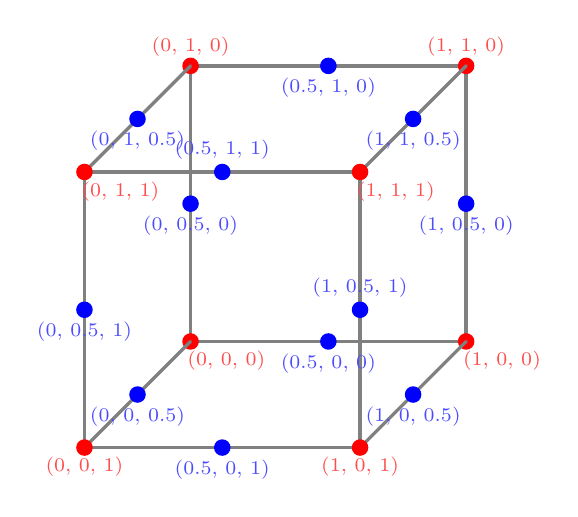
\begin{tikzpicture}[scale=3.5, line join=round, line cap=round]

        % Cube edges
        \draw[gray, very thick] (0,0,0) -- (1,0,0) -- (1,1,0) -- (0,1,0) -- cycle;
        % Vertices (corners)
        \foreach \x/\y/\z in {0/0/0, 1/0/0, 1/1/0, 0/1/0} {
            \fill[red] (\x,\y,\z) circle (0.03);
        }
        \draw[gray, very thick] (0,0,0) -- (0,0,1);
        \draw[gray, very thick] (1,0,0) -- (1,0,1);
        \draw[gray, very thick] (1,1,0) -- (1,1,1);
        \draw[gray, very thick] (0,1,0) -- (0,1,1);
        \draw[gray, very thick] (0,0,1) -- (1,0,1) -- (1,1,1) -- (0,1,1) -- cycle;

       % Vertices (corners)
       \foreach \x/\y/\z in {0/0/1, 1/0/1, 1/1/1, 0/1/1} {
            \fill[red] (\x,\y,\z) circle (0.03);
        }

        % Vertices (Face centers)
        \foreach \x/\y/\z in {0.5/0/0, 0.5/1/0, 0.5/0/1, 0.5/1/1, 0/0.5/0, 1/0.5/0, 0/0.5/1, 1/0.5/1, 0/0/0.5, 1/0/0.5, 0/1/0.5, 1/1/0.5} {
            \fill[blue] (\x,\y,\z) circle (0.03);
        }

        % coordinates (corners)
       \foreach \x/\y/\z in {0/0/1, 1/0/1} {
            \node[red!70!white, font=\scriptsize] at (\x,\y-0.07,\z) {(\x, \y, \z)};
        }
        % coordinates (corners)
       \foreach \x/\y/\z in {0/0/0, 1/0/0, 1/1/1, 0/1/1} {
            \node[red!70!white, font=\scriptsize] at (\x+0.13,\y-0.07,\z) {(\x, \y, \z)};
        }
         % coordinates (corners)
        \foreach \x/\y/\z in {1/1/0, 0/1/0} {
            \node[red!70!white, font=\scriptsize] at (\x,\y+0.07,\z) {(\x, \y, \z)};
        }

        % coordinates (Face centers)
        \foreach \x/\y/\z in {0.5/0/0, 0.5/1/0, 0.5/0/1, 0/0.5/0, 1/0.5/0, 0/0.5/1, 0/0/0.5, 1/0/0.5, 0/1/0.5, 1/1/0.5} {
            \node[blue!70!white, font=\scriptsize] at (\x,\y-0.08,\z) {(\x, \y, \z)};
        }
         % coordinates (Face centers)
         \foreach \x/\y/\z in {0.5/1/1, 1/0.5/1} {
            \node[blue!70!white, font=\scriptsize] at (\x,\y+0.08,\z) {(\x, \y, \z)};
        }
    \end{tikzpicture}

    \caption{Coordonnées des noeuds dans une maille cubique toutes faces centrées.}
    \label{fig:maille}
\end{wrapfigure}

Informations minimum pour représenter une maille.
On retire toutes les coordonnées pouvant être obtenues par translations entières (l'origine du repère n'a aucune importance).
On a besoin d'autant de coordonnées que de nombre d'espèces appartenant en propre à la maille.

\vspace{3mm}
\noindent\textbf{Les coordonnées réduites sont alors:}
\vspace{3mm}
\begin{itemize}[label=$\ast$]
    \item \textcolor{red}{\Large $\left(0, 0, 0\right)$}.
    \item \textcolor{blue}{\Large $\left(\nicefrac{1}{2}, 0, 0\right), \left(0, \nicefrac{1}{2}, 0\right), \left(0, 0, \nicefrac{1}{2}\right)$}
\end{itemize}

\vspace{0.8cm}

\subsubsection{Remarques}

\noindent Plusieurs informations utiles pour les exercices:
\begin{itemize}[label=$\ast$]
    \item Métal $\quad \rightarrow \quad$ tangence
    \item Empilement compact $\quad \rightarrow \quad \mathcal{C} = 0.74$
    \item Empilement semi-compact $\quad \rightarrow \quad \mathcal{C} = 0.68$
    \item Maille électriquement neutre $\quad \rightarrow \quad$ autant de cation que d'anion dans Na$^+$Cl$^-$ par exemple.
    \item $\text{Composition motif} = \dfrac{\text{contenu maille}}{\text{nb noeuds}}$
    \item Formule très utile: $\rho = \dfrac{m}{V_{\text{maille}}} = \dfrac{M_X n_X}{a^3} = \dfrac{M_X N_X}{\mathcal{N}a^3}$
\end{itemize}


\subsection{Cas pratique, exercice corrigé}

A l'état solide, le soufre ($M_S = \qty{32.06}{g.mol^{-1}}$, $\rho = \qty{2.087}{g.cm-3}$)
est constitué de molécules cycliques de formule $S_8$ et forme des cristaux jaunes appartenant au système orthorhombique 
($\alpha=\beta=\gamma=90^{\circ}$). Les paramètres cristallins, déterminés par une
étude radiocristallographique, ont pour valeurs:
$$a = \qty{10.437}{\angstrom} \quad b = \qty{12.845}{\angstrom} \quad c = \qty{24.369}{\angstrom}$$ 

\vspace{5mm}\noindent \textit{a) Quelle serait la composition du motif en nombre de molécules $S_8$ de la structure
dans chacun des modes de réseau possibles (primitif P, base centrée S, intérieur centré I et 
toutes faces centrées F) ? }\\
\textit{b) Tracez les axes de symétrie du système orthorhombique. Préciser l'ordre de symétrie des axes.}

\vspace{5mm}\noindent\textbf{Réponses:}

\textbf{a)} $\quad \text{Composition motif} = \dfrac{\text{contenu maille}}{\text{nb noeuds}}$

$\quad \rho_{\text{soufre}} = \dfrac{8 M_S N_{S_8}}{\mathcal{N}(a b c)^3}
\quad \Longleftrightarrow \quad N_{S_8}= \dfrac{\mathcal{N}\rho_{\text{S}(abc)^3}}{8M_S} = 16 \quad$
Ainsi il y a 16 $S_8$ par maille.

Le nombre de noeuds dépend du mode de réseau: (P: 1), (S: 2), (I: 2) ou (F: 4).
$$\text{Motif:} \quad (P) = \frac{16}{1}=16 \quad (S) = \frac{16}{2}=8 \quad (I) = \frac{16}{2}=8 \quad (F) = \frac{16}{4}=4$$



\clearpage

\begin{figure}[H]
    \centering
    \vspace{-0.5cm}
    \begin{subfigure}{0.3\textwidth}
        \centering
        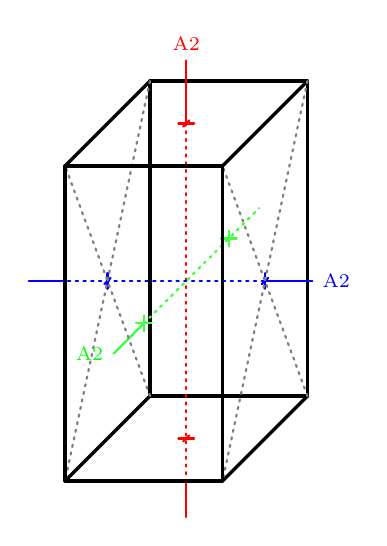
\begin{tikzpicture}[scale=2, line join=round, line cap=round]

            % Définir les sommets d'un cube
            \coordinate (A) at (0, 0, 0);
            \coordinate (B) at (1, 0, 0);
            \coordinate (C) at (1, 2, 0);
            \coordinate (D) at (0, 2, 0);
            \coordinate (E) at (0, 0, 1.4);
            \coordinate (F) at (1, 0, 1.4);
            \coordinate (G) at (1, 2, 1.4);
            \coordinate (H) at (0, 2, 1.4);
                
            \draw[black, very thick] (A) -- (B) -- (C) -- (D) -- cycle; % Face de derriere
            
            % Axe d'ordre 4 (centre de deux faces opposées)
            \draw[red, thick, dotted] (0.5, 2, 0.7) -- (0.5, -0.3, 0.7);
            \draw[red, thick] (0.5, -0.5, 0.7) -- (0.5, -0.28, 0.7);
            \draw[red, thick] (0.5, 2, 0.7) -- (0.5, 2.4, 0.7) node[above, red] {\scriptsize A2};
            \draw[red, thick] (0.5, 0, 0.65) -- (0.5, 0, 0.75); % cross
            \draw[red, thick] (0.45, 0, 0.7) -- (0.55, 0, 0.7); % cross
            \draw[red, thick] (0.5, 2, 0.65) -- (0.5, 2, 0.75); % cross
            \draw[red, thick] (0.45, 2, 0.7) -- (0.55, 2, 0.7); % cross
    
             % Axe d'ordre 4 (centre de deux faces opposées)
             \draw[blue, thick, dotted] (-0.3, 1, 0.7) -- (1, 1, 0.7);
             \draw[blue, thick] (-0.3, 1, 0.7) -- (-0.5, 1, 0.7);
             \draw[blue, thick] (1, 1, 0.7) -- (1.3, 1, 0.7) node[right, blue] {\scriptsize A2};
             \draw[blue, thick] (0, 1, 0.65) -- (0, 1, 0.75); % cross
             \draw[blue, thick] (0, 1.05, 0.7) -- (0, 0.95, 0.7); % cross
             \draw[blue, thick] (1, 1, 0.65) -- (1, 1, 0.75); % cross
             \draw[blue, thick] (1, 1.05, 0.7) -- (1, 0.95, 0.7); % cross
        
             % Axe d'ordre 4 (centre de deux faces opposées)
             \draw[green!75, thick, dotted] (0.5, 1, 1.4) -- (0.5, 1, -0.5);
             \draw[green!75, thick] (0.5, 1, 1.4) -- (0.5, 1, 1.9) node[left, green] {\scriptsize A2};
             \draw[green!75, thick] (0.45, 1, 0) -- (0.55, 1, 0); % cross
             \draw[green!75, thick] (0.5, 0.95, 0) -- (0.5, 1.05, 0); % cross
             \draw[green!75, thick] (0.45, 1, 1.4) -- (0.55, 1, 1.4); % cross
             \draw[green!75, thick] (0.5, 0.95, 1.4) -- (0.5, 1.05, 1.4); % cross
    
    
             \draw[black, very thick] (A) -- (E); % Arêtes verticales
             \draw[black, very thick] (B) -- (F);
             \draw[black, very thick] (C) -- (G);
             \draw[black, very thick] (D) -- (H);
    
             % diagonale
             \draw[gray, thick, dotted] (D) -- (E);
             \draw[gray, thick, dotted] (B) -- (G);
             \draw[gray, thick, dotted] (C) -- (F);
             \draw[gray, thick, dotted] (A) -- (H);
    
            % Tracer les arêtes du cube
            \draw[black, very thick] (E) -- (F) -- (G) -- (H) -- cycle; % Face supérieure
        
        \end{tikzpicture}
        \caption{Axes de symétries du système orthorhombique}
        \label{fig:symetrie orthorhombique}
    \end{subfigure}
    \hfill\vspace{-0.5cm}\begin{subfigure}{0.3\textwidth}
        \centering
        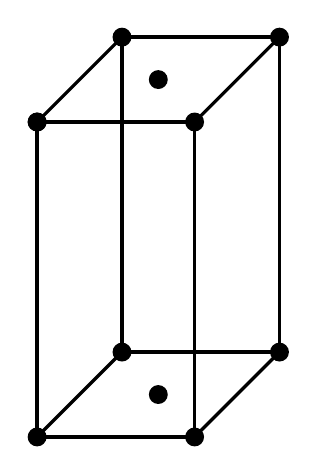
\begin{tikzpicture}[scale=2, line join=round, line cap=round]

            % Définir les sommets d'un cube
            \coordinate (A) at (0, 0, 0);
            \coordinate (B) at (1, 0, 0);
            \coordinate (C) at (1, 2, 0);
            \coordinate (D) at (0, 2, 0);
            \coordinate (E) at (0, 0, 1.4);
            \coordinate (F) at (1, 0, 1.4);
            \coordinate (G) at (1, 2, 1.4);
            \coordinate (H) at (0, 2, 1.4);
                
            \draw[black, very thick] (A) -- (B) -- (C) -- (D) -- cycle; % Face de derriere
             \draw[black, very thick] (A) -- (E); % Arêtes verticales
             \draw[black, very thick] (B) -- (F);
             \draw[black, very thick] (C) -- (G);
             \draw[black, very thick] (D) -- (H);
            % Tracer les arêtes du cube
            \draw[black, very thick] (E) -- (F) -- (G) -- (H) -- cycle; % Face supérieure
            
            % Vertices of the cube (foreground)
            \foreach \x/\y/\z in {0/0/1.4, 1/0/1.4, 1/2/1.4, 0/2/1.4, 0/0/0, 1/0/0, 0/2/0, 0/2/1.4, 1/2/0, 0.5/0/0.7, 0.5/2/0.7} {
                \fill[black] (\x,\y,\z) circle (0.06);
            }
            
        \end{tikzpicture}

        \caption{orthorhombique base centré}
        \label{orthorhombique base centre}
    \end{subfigure}
\end{figure}

\vspace{8mm}
\hrule
\vspace{3mm}
\begin{figure}[H]
    \centering
    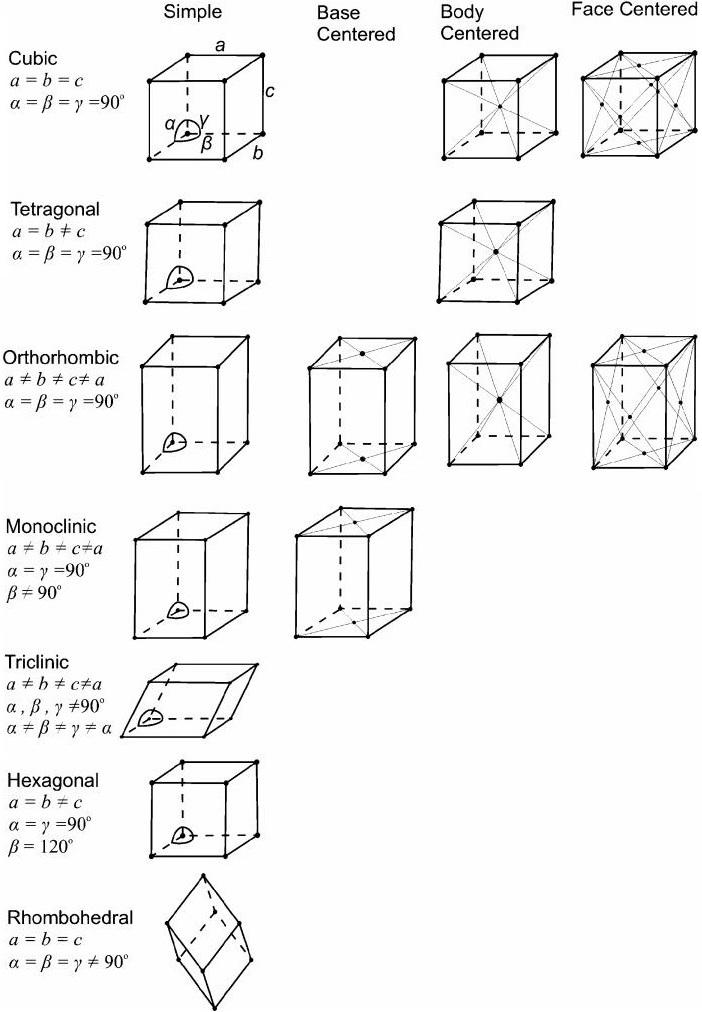
\includegraphics[width=0.65\textwidth]{Fig/bravais.jpg}
    \caption{Les 7 systèmes cristallins et les 14 réseaux de Bravais}
    \label{fig:bravais}
\end{figure}


\section{Formulaire, Constantes et Unités}

\subsection{Formules}

\begin{itemize}[label=$\ast$]
    \item \textbf{Conversion d'Energie:}
    $$E_{eV}=\frac{E_J}{\qty{1.602e-19}{}} \Longleftrightarrow E_J=E_{eV}\times \qty{1.602e-19}{}$$

    \item \textbf{Ritz-Balmer généralisée} (pour les hydrogénoïdes):
    $$\frac{1}{\lambda} = Z^2R_X \left(\frac{1}{n'^2}-\frac{1}{n^2}\right)$$
\hfill $n,n'\in \mathbb{N} \text{\quad tels que\quad} n'<n$.

\item \textbf{Relation liant $\bm{E}$, $\bm{\nu}$ et $\bm{\lambda}$:} $$E=h\nu=\frac{hc}{\lambda}$$ 

\item \textbf{Loi de Moseley:} $$\sqrt{\nu}=a(Z-b)=AZ+B$$

\item \textbf{Loi de Beer Lambert:} $$I=I_0 \exp{(-\mu x)}$$

\item \textbf{Charge effective:} $$Z^*_i=Z-\sigma_i$$

\item \textbf{Règles de Slater:} \newline
Contributions des électrons des orbitales $n'$ à la constante d'écran $\sigma$  agissant sur un électron donné d'une orbitale $n$.
\vspace{5mm}
\resttable %duplicate the Slater table defined above

\end{itemize}


\subsection{Constantes et Unités}

\begin{table}[h]
\centering
    \begin{tabular}{|c|c|c|}
    \hline
        \textbf{Symboles} & \textbf{Noms} & \textbf{Valeurs} \\ \hline
        $\mathcal{N}$ & Nombre d'Avogadro & $\approx \qty{6.022e23}{mol^{-1}}$ \\ \hline
        $\bm{e}$ & Charge élémentaire & $\approx \qty{1.602e-19}{\coulomb}$ \\ \hline
        $\bm{m_e}$ & Masse de l'électron au repos & $\approx \qty{9.109e-31}{kg}$ \\ \hline
        $\bm{h}$ & Constante de Plank & $\approx \qty{6.626e-34}{Js}$ \\ \hline
        $\bm{R_h}$ & Constante de Rydberg pour l'hydrogène & $\approx \qty{109677.80}{cm^{-1}}$ \\ \hline
        $\bm{R_\infty}$ & Constante de Rydberg pour un noyau de masse infinie & $\approx \qty{109737.31}{cm^{-1}}$ \\ \hline
        $\bm{c}$ & Vitesse de la lumière dans le vide & $\approx \qty{2.998e8}{ms^{-1}}$ \\ \hline    
    \end{tabular}
    \caption{Constantes Fondamentales}
    \label{tab:Constantes Fondamentales}
\end{table}    


\begin{landscape} % begin on a new page
    % First periodic table
    \begin{center}{
        \normalfont\Large\bfseries Électronégativité des éléments du Tableau Périodique}
    \end{center} % removed \section to avoid creating another new page
    
    \pagestyle{empty}  % Remove headers and footers for the landscape section

    \pgfPTbuildcell(5,3)[(1;1-2;Z),(2;1-3;CS),(3-4;1-3;eneg),(5;1-3;name)]
    \vspace{-5mm}
    \hspace{-2cm}\pgfPT[
        show title=false, 
        csSoft,                               % General style of the periodic table
        show legend=true, 
        Z={bc={lightgray},f=\normalsize\bfseries\itshape}, % set the color of the Z bg and size
        Z color=black, 
        Z align=center, 
        CS font=\large\bfseries,
        name font=\scriptsize,
        CS render mode=fill, 
        CS synt=pink, 
        cell size=42pt,
        group numbers=CAS, % group numbers in Roman numerals
        Roman label color=black,
        period label color=black,
        MNM line width=1pt,
        eneg font=\large\bfseries,
        eneg color=red
        ]
    \footnote{Retourner à la sous-section \ref{sous-section:Electronégativité}.}
\end{landscape}

\begin{landscape} % begin on a new page
    % Second periodic table
    \section*{\centering Tableau Périodique des Éléments}
    \thispagestyle{empty}  % Remove headers and footers for the landscape section

    \pgfPTbuildcell(5,3)[(1;1-2;Z),(2-3;1-3;CS),(4-5;1-3;name)]
    \hspace{-2cm}\pgfPT[
        show title=false, 
        csSoft,                               % General style of the periodic table
        show legend=true, 
        Z={bc={lightgray},f=\normalsize\bfseries\itshape}, % set the color of the Z bg and size
        Z color=black, 
        Z align=center, 
        CS font=\Large\bfseries,
        name font=\scriptsize,
        CS render mode=fill, 
        CS synt=pink, 
        cell size=42pt,
        group numbers=CAS, % group numbers in Roman numerals
        Roman label color=black,
        period label color=black,
        MNM line width=2pt
        ]

\end{landscape}

\end{document}